\documentclass[12pt,letterpaper,chap,twoside]{thesis}
%agragar comentario
%Tesis modificada desde linux (fedora) Utilizando git y github(cuenta)
\usepackage[utf8]{inputenc}
%\usepackage[latin1]{inputenc}
\usepackage[T1]{fontenc}
\usepackage[english,spanish,es-tabla]{babel}
\usepackage{listings}
\usepackage{mathptmx}
\usepackage{textcomp}
\usepackage{amsmath}
\usepackage{amsfonts}
\usepackage{amssymb}
\usepackage{imakeidx}
\usepackage{graphicx}
\usepackage{subfigure}
\usepackage{enumerate}
\usepackage{tocbibind}
\usepackage{hyperref}
%\usepackage{natbib,har2nat}
\usepackage{pdfpages}
\usepackage{multicol}
\hypersetup{
	pdftitle={Tesis},
	pdfauthor={Iván Zamora Ramírez},
	pdfsubject={Your subject here},
	pdfkeywords={monocromador, PMT},
	bookmarksnumbered=true,     
	bookmarksopen=true,         
	bookmarksopenlevel=1,       
	colorlinks=true,            
	pdfstartview=Fit,           
	pdfpagemode=UseOutlines,    % this is the option you were lookin for
	pdfpagelayout=TwoPageRight
}
\hypersetup{pdftex,colorlinks=true,allcolors=black}
\usepackage{hypcap}
\usepackage{bookmark}
%\usepackage[hang]{caption}
%\renewcommand{\captionfont}{\bfseries}
%\usepackage[left=3.0cm, right=2.5cm, top=2.5cm, bottom=2.5cm]{geometry}
%\makeindex % para que cree el índice (pero aún no decimos dónde)
\begin{document}
	\renewcommand{\shorthandsspanish}{}
	\renewcommand{\listtablename}{Índice de tablas} 
	\renewcommand{\tablename}{Tabla} 
	
% Supply information for use on title page:
\begin{picture}(0,0) \put(-10,-90){
\includegraphics[width=20mm]{Imagenes/escudo}} \end{picture}
\begin{picture}(0,0) \put(-10,-550){
\includegraphics[width=30mm]{Imagenes/ESIME}} \end{picture}
\institute{INSTITUTO POLITÉCNICO NACIONAL}
\school{ESCUELA SUPERIOR DE INGENIERÍA \\ MECÁNICA Y ELÉCTRICA}
\unidad{DE ESTUDIOS DE POSGRADO E INVESTIGACIÓN}
\thesistitle{\textbf{"Desarrollo de un sistema espectrométrico automatizado".}}        
\author{Ing. Iván Zamora Ramírez}        

\degree{Maestría en Ciencias en Ingeniería Electrónica} 

\department{Fotónica} % provide your area of study here; e.g.,
%  "Mechanical Engineering", "Nuclear Engineering", "Physics", etc.
\setlength{\unitlength}{2pt}

%\signaturelines{3}
%\thadviser{Dr. José Manuel de la Rosa Vázquez} % For a masters project use \projadviser instead of \thadviser,
\memberone{Dr. José Manuel de la Rosa Vázquez}        
\membertwo{Dr. Suren Stolik Isakina}
%\memberthree{Aristotle} % must change signaturelines to 4 if using this 4 members

\submitdate{Ciudad de México, 2019 }        
\copyrightyear{2019}   % if omitted, current year is used.        
\titlepage     
\newpage{\ } 

	\specialhead{Dedicatoria}
\begin{flushright}
    Que tus segundos se llenen de magia.\\
    que tus minutos de risa.\\
    Que tus horas de amor.\\
    Y en tu corazón; la paz, la esperanza y el perdon. 

    Gracias madre por todo lo que me diste. \\ 
    Tú siempre seguiras aquí conmigo, con nosotros. 
    	
\end{flushright} 
	\specialhead{Agradecimientos}
... 	
	\tableofcontents
\listoffigures
\listoftables
\specialhead{Resumen}
La espectroscopia es una técnica de medición para estudiar la interacción de la radiación electromagnética con la materia.
Dentro del amplio espectro electromagnético, el presente trabajo se enfocará en la luz ultravioleta (UV) y la luz visible (VIS). Hoy en día existen en el mercado equipos capaces de realizar espectroscopia óptica, sin embargo, la mayoría tienen costos elevados. Aprovechando equipo de laboratorio con el cual se cuenta, se ha desarrollado un sistema espectroscópico automatizado. \\
El sistema consta de un monocromador SpectraPro 275, un módulo de tubo fotomultiplicador (PMT) y un motor a pasos. Los cuáles serán controlados por un microcontrolador y una PC.\\
El intervalo de trabajo de este espectrómetro es de los 200 hasta los 650nm, con un paso promedio de 0.05nm. \\
La Interfaz gráfica fue diseñada en LabView, se utilizó un microcontrolador para el control y un ADC para la adquisición de los datos.

	\begin{otherlanguage}{english}
\specialhead{Abstract}
The spectroscopy is a measurement technique to study the interaction of electromagnetic radiation with matter.
Within the broad electromagnetic spectrum, this work is focused on ultraviolet light (UV) and visible light (VIS). Nowadays there are equipment avaible on the market capable of performing automated optical spectroscopy however, it is expensive. Using available  laboratory equipment, an automated spectroscopic system has been developed. \\
The system consists of a SpectraPro 275 monochromator, a photomultiplier tube (PMT) module and a stepper motor. The system is controlled by a microcontroller and a PC. \\
The wavelength working range of this spectrometer is from 200 to 650 nm, with an average step of 0.05 nm. \\
The Graphical User Interface (GUI) was designed in LabView, a microcontroller was used to control the system and an analog to digital converter (ADC) to data acquisition.

\end{otherlanguage}{}
	\chapter*{Hipótesis}
%Es posible automatizar y calibrar un monocromador usando un motor a pasos y una PC. 
Es posible a partir de un monocromador y utilizando un sistema de motor a pasos y un fotomultiplicador diseñar, construir y caracterizar un espectrómetro automatizado y controlado por una PC.
\addcontentsline{toc}{chapter}{Hipótesis}
	\specialhead{Justificación}
La línea de investigación de instrumentación fotónica de la SEPI-ESIME-Z cuenta con diversos miniespectrómetros para la realización de sus investigaciones. Estos miniespectrómetros permiten en principio la captura automática de espectros de luz continua  con resoluciones de hasta 0.5 nm. El automatizar un monocromador permitirá realizar, además de espectroscopia de luz continua, espectroscopia resuelta en tiempo y de mucha más alta resolución.


Al ser un sistema desarrollado en el propio laboratorio, este podrá ser modificado con facilidad con la finalidad de mejorar sus características o para aplicaciones particulares. Otro de los beneficios que se obtiene con automatizar el monocromador, es el bajo costo que esto implica en comparación con la compra de un sistema comercial automatizado. Con el sistema propuesto se podrá además:
\begin{itemize}
\item Estudiar fuentes luminosas de baja intensidad.
\item Podrá ser modificado para realizar mediciones en otros intervalos del espectro de luz con el cambio de la rejilla de difracción y el tubo fotomultiplicador.
\end{itemize}

\paragraph{Aplicaciones} 
El monocromador tiene un alto poder de resolución, al combinarlo con un tubo fotomultiplicador de alta sensibilidad, será posible medir espectros de emisión de los plasmas estudiados en el grupo de instrumentación fotónica.

	\chapter*{Objetivo General}
Diseñar y caracterizar un espectrómetro de alta resolución y alta sensibilidad utilizando un monocromador, Acton Research Corportion Spectrapro 275,  un módulo de tubo fotomultiplicador y un motor a pasos.
\addcontentsline{toc}{chapter}{Objetivo General} % para que lo añada al índice de contenidos
\section*{Objetivos Particulares}
\begin{itemize}
\item Diseñar un sistema para seleccionar la longitud de onda mediante el control de la posición angular de la red de difracción.

\item Desarrolar una interfaz gráfica para controlar el sistema y observar los espectros medidos.

\item Calibrar el espectrómetro utilizando una lámpara de mercurio.

\item Desarrollar un sistema de control de la ganancia del tubo fotomultiplicador.

\item Comparar las mediciones del sistema propuesto con los miniespectrómetros comerciales de Ocean Optics con los que cuenta la línea de instrumentación fotónica de la SEPI-ESIMEZ.
\end{itemize}
\addcontentsline{toc}{section}{Objetivos Particulares} % para que lo añada al índice de contenidos
	\pagenumbering{arabic}
	\chapter{Introducción}
El presente trabajo de tesis está dedicado al diseño, construcción, caracterización e implementación de un sistema automatizado para la realización de estudios de espectroscopia, UV-VIS, utilizando un monocromador como sistema para descomponer la luz  en sus diferentes longitudes de onda y un tubo fotomultiplicador (PMT) para medir la potencia radiante de cada una.

La espectroscopia óptica es una herramienta utilizada para el estudio de materiales a partir de la medición de la luz absorbida o emitida por la materia, El intervalo del espectro electromagnético que el sistema permitirá estudiar parte de los 200 nm hasta los 700 nm (Ultravioleta medio, ultravioleta cercano y luz visible). En la figura \ref{fig:espectrovisible} se observa el espectro electromagnético, se presenta una ampliación del espectro visible (VIS) el cual abarca un intervalo muy pequeño dentro de todo el espectro electromagnético. 
\begin{figure}[h!]%figura 1
	\centering
	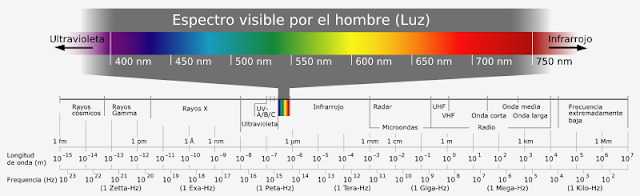
\includegraphics[width=1\linewidth]{Imagenes/espectro_visible}
	\caption[Espectro electromagnético, enfatizando el espectro visible para el ojo humano \cite{espectroOjo}.]{Las ondas electromagnéticas se clasifican en rayos-$\gamma$(gamma), rayos-x, ultravioleta, luz visible, infrarrojos, microondas y ondas de radio. En la figura se enfatiza en el espectro visible (VIS) para el ojo humano \cite{espectroOjo}}
	\label{fig:espectrovisible}
\end{figure}

\section{Espectro electromagnético.}
Se denomina espectro electromagnético a la representación de la distribución energética de las ondas electromagnéticas respecto a la longitud de onda o de su frecuencia. El espectro de la radiación electromagnética que emite o absorbe un objeto depende de su composición y de su temperatura. Dicha radiación nos brinda información sobre la materia y sirve para identificar las sustancias presentes, ya que el espectro es único para cada sustancia de manera similar a una huella dactilar. 
\begin{figure}[h!] %figura 2
	\centering
	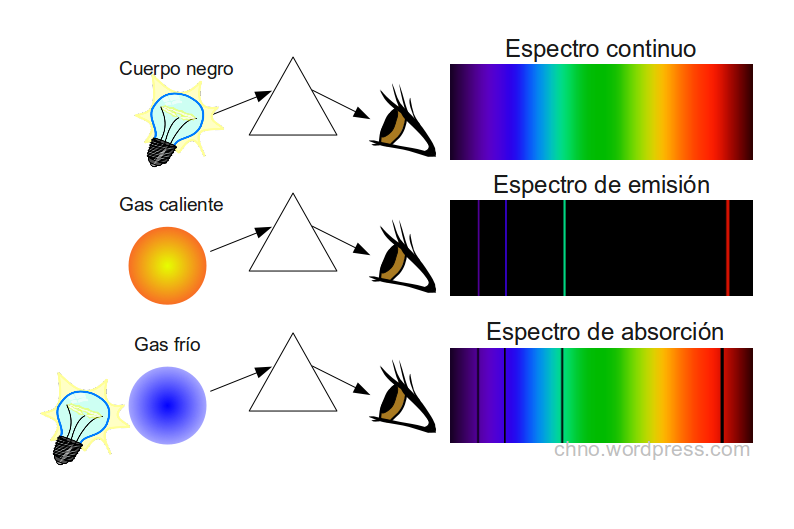
\includegraphics[width=1\linewidth]{Imagenes/espectros_absorcion_y_emision}
	\caption{Tipos de espectros. \cite{FisicaCh}}
	\label{fig:esq_espectro01}
\end{figure}

En la figura \ref{fig:esq_espectro01} se observan diferentes espectros y cómo se producen estos, donde el primero, es el espectro continuo o de cuerpo negro, en el cuál se observa una banda continua. Es emitido por cualquier objeto caliente, el espectro solar es un ejemplo de este. El espectro de emisión de líneas es generado cuando los átomos y moléculas en un gas caliente emiten una radiación en ciertas longitudes de onda. Por otra parte el espectro de absorción se observa cuando el mismo gas, recibe radiación electromagnética, este gas absorbería ciertas longitudes de onda. Se observa que las líneas emitidas son las mismas que las que no se presentan cuando absorbe. Cumpliendo con esto la ley de Kirchhoff de la radiación térmica: \emph{si un cuerpo (o superficie) está en equilibrio termodinámico con su entorno, su emisividad $\epsilon$ es igual a su absortividad $\alpha$} .

\subsection{Intervalo energético del espectro.}
El espectro electromagnético cubre un intervalo de frecuencias (o longitudes de onda) muy amplio. Las frecuencias desde 30 HZ y menores que son relevantes en el estudio de ciertas nebulosas. Por otro lado,los rayos cósmicos presentanfrecuencias cercanas a los  $2.9 \times 10^{27}$ Hz.
La energía que porta la onda electromagnética está relacionada con el cuadrado de la amplitud de la intensidad del campo eléctrico. 

La dualidad onda-particula permite que la radiación electromagnética pueda ser descrita con modelos diferentes, como una onda y como un flujo de partículas, fotones. Este fotón tendrá una energia E directamente proporcional a la frecuencia de la onda que le corresponde. La relación es 
$\lambda = c/f$. La energía de un fotón está dada por la siguiente ecuación.
\begin{equation}
E = hf =h\cdot \frac{c}{\lambda}
\label{equa:intcuad}
\end{equation}
\begin{itemize}
	\item $h$ constante de Planck, $h \approx 6.626069\times 10^{34} J\cdot s$.
	\item $\lambda$ longitud de onda en ($nm$).
	\item $f$ frecuencia de la luz ($Hz$).
	\item c velocidad de la luz en el vacío $c = \frac{1}{\sqrt{\mu_0\epsilon_0}}$, $c = 299,792,458 m/s$
	\subitem $\mu_0$ permeabilidad en el vacío $\mu_0 = 4\pi\times10^{-7} N\cdot A^{-2}$
	\subitem $\epsilon_0$ es la permitividad en el vacío $\epsilon_0 = 8.85418\times10^{12} C^2/N\cdot m^2$
	
\end{itemize}
Podemos reescribir la ecuación \ref{equa:intcuad}, expresando la energía $E$ en $eV$, la longitud de onda en nanómetros ($nm$), $1eV = 1.6\times 10^{-19} J$
\begin{equation}
E(ev)\approx \frac{1240}{\lambda}
\label{equa:intcuad2}
\end{equation}
De modo que para un fotón que corresponde a una longitud de onda igual a 200nm se tiene una energía de 6.2eV mientras que para uno que corresponda a una longitud de onda de 700nm la energía será de 1.77eV.
$$E_{200}\approx \frac{1240}{200}=6.2eV $$
$$E_{700}\approx \frac{1240}{700}=1.77eV $$
De la ecuación \ref{equa:intcuad2} podemos observar la energía es inversamente proporcional a la longitud de onda, a longitudes de onda menores tendremos mayor energía, y a mayores longitudes de onda menor energía.
Las ondas electromagnéticas se clasifican en: rayos-$\gamma$, rayos-x, ultravioleta, luz visible, infrarrojos, microondas y ondas de radio.

\subsection{Región visible}
El intervalo de luz visible va desde los 400nm hasta los 700nm aproximadamente, se le llama así a esta región por ser el intervalo donde el ojo humano tiene sensibilidad, ver figura \ref{fig:ojohumano}. La máxima sensibilidad del ojo humano se encuentra a los 555nm (verde) para luz diurna, la respuesta espectral del ojo humano fue establecida por la CIE, Commission internationale de l'éclairage \cite{CIE1924}.

En la tabla \ref{tabla:ojo},  se observan los intervalos en longitud de onda para los colores que componen la luz blanca.
Newton fue el primero en establecer que la luz blanca está compuesta de todos los colores del espectro visible.
\begin{figure}
	\centering
	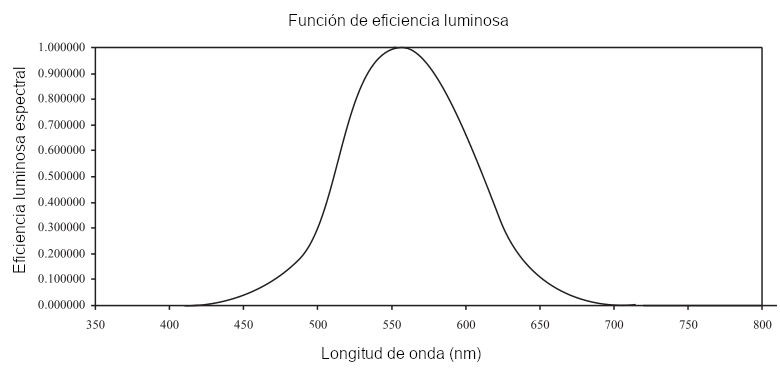
\includegraphics[width=0.8\linewidth]{Imagenes/SpectralL}
	\caption{Sensibilidad del ojo humano ante el espectro electromagnético, \cite{CRC2016}, \cite{inproceedings}}
	\label{fig:ojohumano}
\end{figure}

\begin{table}
\centering

\caption{Intervalos de longitud de onda en el vacío para los distintos colores. \cite{Bruno2005}}
\begin{tabular}{|c|c|}
	\hline 
	Color & $\lambda$ Longitud de onda ($nm$) \\ 
	\hline 
	Violeta & 380-450 \\ 
	\hline 
	Azul & 450-495  \\ 
	\hline 
	Verde & 495-570  \\ 
	\hline 
	Amarillo & 570-590 \\ 
	\hline 
	Naranja & 590-620 \\ 
	\hline 
	Rojo & 620-750 \\ 
	\hline 
\end{tabular} 
\label{tabla:ojo}		
\end{table}


\subsection{Ultravioleta}
La luz ultravioleta es el intervalo del espectro electromagnético que va desde los 10nm hasta los 400nm, se puede dividir en varios intervalos definidos por la \textbf{ISO 21348} \cite{Solar}. En la tabla \ref{tabla:UV} se muestran las subcategorías para el ultravioleta. En este trabajo utilizaremos las subcategorías NUV y MUV (200-400 $nm$). 
\begin{table}
	\centering
	\caption{ISO 21348 sección de subcategorías del ultravioleta. \cite{Solar}} 
	\label{tabla:UV}
	\begin{tabular}{|c c c|}
		\hline
		Subcategoria UV & Intervalo en \textbf{$nm$} & Descripción. \\
		\hline
		UV & 10$\leq\lambda\leq$400 & Ultravioleta \\
		\hline
		\hline
		UVA & 315$\leq\lambda\leq$400 & Ultravioleta A\\
		UVB & 280$\leq\lambda\leq$315 & Ultravioleta B\\
		UVC & 100$\leq\lambda\leq$280 & Ultravioleta C\\
		\hline
		\hline
		NUV & 300$\leq\lambda\leq$400 & Ultravioleta cercano\\
		MUV & 200$\leq\lambda\leq$300 & Ultravioleta medio\\
		FUV & 122$\leq\lambda\leq$200 & Ultravioleta lejano\\
		H-Lyman-$\alpha$ & 121$\leq\lambda\leq$122 &  linea Lyman alfa\\
		\hline\hline
		VUV & 10$\leq\lambda\leq$200 & Ultravioleta de vacío\\
		EUV & 10$\leq\lambda\leq$121 & Ultravioleta extremo.\\
		\hline
	\end{tabular}
\end{table}

\section{Espectrometría.}
La interacción de la radiación electromagnética con la materia se puede describir a partir del cambio de la distribución de intensidad de la radiación electromagnética, emitida o absorbida, por una sustancia, en función de su longitud de onda. Al analizar la radiación emitida o absorbida por la materia, se pueden identificar las sustancias que la componen. 


\section{Espectrómetro}
El espectrómetro óptico es un instrumento utilizado para analizar la luz, para esto, el espectrómetro descompone la luz a estudiar en sus diferentes longitudes de onda que la componen, y mide la potencia radiante en cada una de estas longitudes de onda. Con lo cual obtendremos una gráfica de la distribución de potencia radiante dependiendo de la longitud de onda. Fig. \ref{fig:espectrosol} \cite{B&WTek2016}. 

\begin{figure}[h!]
	\centering
	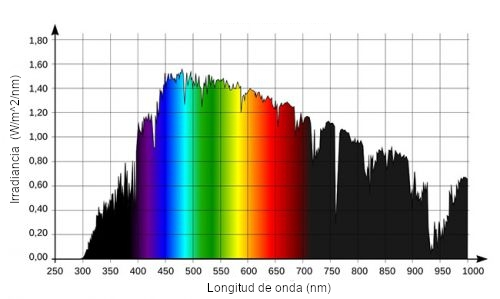
\includegraphics[width=0.9\linewidth,height=5cm]{Imagenes/espectroSOL}
	\caption[Espectro continuo, luz solar \cite{SolarLight}.]{El espectro solar es un ejemplo de espectro continuo, se grafica la irradiancia espectral contra longitud de onda.}
	\label{fig:espectrosol}
\end{figure}
\subsection{Funcionamiento de espectrómetro.}
%El funcionamiento básico del espectrómetro es descomponer la luz en sus componentes espectrales, medir la intensidad de la señal en función de la longitud de onda, y graficar las intensidades medidas en relación con la longitud de onda. 
%\begin{enumerate}[a]
%	\item Ranura de entrada o \textsl{slit}.
%	\item Espejo colimador.
%	\item Red de difracción.
%	\item Detector
%\end{enumerate}

El primer paso es introducir la luz al espectrómetro, la luz entra por una pequeña apertura, \textbf{la ranura de entrada}, ver la figura \ref{fig:esquematicoespectrometro}(a). Aquí la luz diverge, esta luz es colimada utilizando un \textbf{espejo cóncavo} figura \ref{fig:esquematicoespectrometro}(b) y reflejada hacia la \textbf{red de difracción} figura \ref{fig:esquematicoespectrometro}(c). Aquí ocurre el fenómeno de difracción separando la luz en sus diferentes componentes espectrales, cada componente espectral se refleja en un ángulo diferente, mas adelante en la ecuación \ref{equa:RedDifra} se describe este fenómeno.  %$m\lambda = d(sin(\alpha)+sin(\beta)) $. 
Las componentes son enfocadas por un segundo \textbf{espejo cóncavo} figura \ref{fig:esquematicoespectrometro}(d), al final son proyectadas en el \textbf{detector} figura \ref{fig:esquematicoespectrometro}(e). La señal luminosa es entonces convertida a una señal eléctrica. Como ejemplo tenemos los miniespectrómetros de Ocean Optics que con base en la dispersión lineal
de la red de difracción y los pixeles en el detector (CCD), el software (propio del espectrómetro) obtiene la relación en
longitud de onda, y así se obtiene un espectro de intensidad en función de la longitud de onda.

\begin{figure}[h]
	\centering
	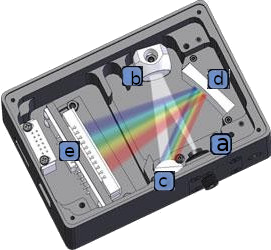
\includegraphics[width=0.55\linewidth]{Imagenes/Espectrometro}
	\caption[Esquema de un espectrómetro.]{Esquemático de un espectrómetro. Se aprecia como la luz es colimada, refractada y enfocada al sensor CCD \cite{BWTEK}}
	\label{fig:esquematicoespectrometro}
\end{figure}

\subsubsection{Ranura de entrada.}
La ranura de entrada o \textit{slit} de entrada, es la entrada de luz al espectrómetro, aquí es donde se define la \textit{cantidad de luz, flujo de fotones}, que entrara en el espectrómetro, fig. \ref{fig:colimarluz} punto (a).
El \textit{slit} es de suma importancia para la resolución óptica del sistema, Normalmente los espectrómetros cuentan con diferentes aperturas de esta ranuras, que van desde los 5$\mu m$ hasta los 200$\mu m$, siendo seis las más comunes: 5$\mu m$, 10$\mu m$, 20$\mu m$, 25$\mu m$, 50$\mu m$, 100$\mu m$ o 200$\mu m$, \cite{Oceana}.

\subsubsection{Espejo colimador.}
Se encarga de hacer que los haces que han pasado por la ranura de entrada sean colimados. Utilizando un espejo cóncavo y teniendo el foco del espejo en la ranura de entrada, hace que todos los haces sean reflejados de forma paralela entre ellos, luz colimada, fig. \ref{fig:colimarluz}, espejo (C). 

\begin{figure}[h]
	\centering
	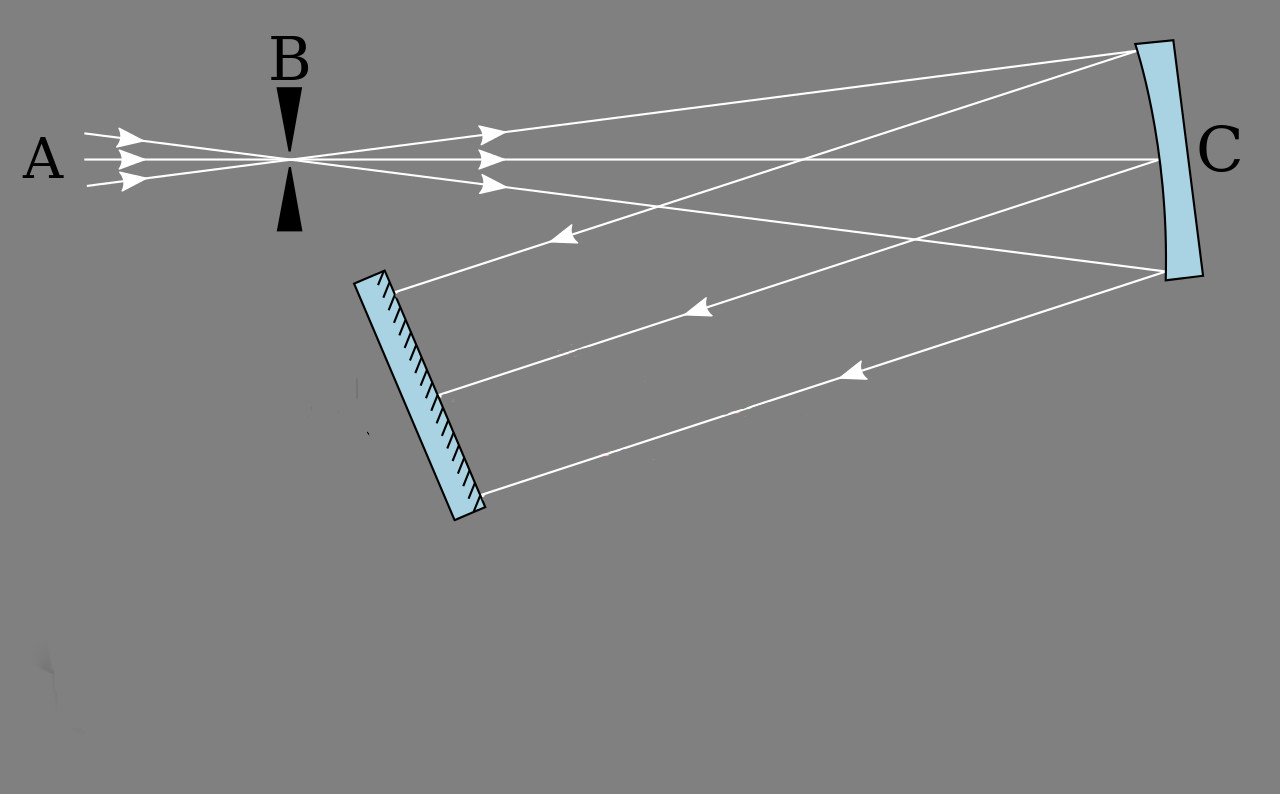
\includegraphics[width=0.6\linewidth]{Imagenes/ColimarLuz}
	\caption{Diagrama óptico de los haces a la entrada del monocromador y colimados hacia la red de difracción. \cite{Czerny-Turney-Conf}}
	\label{fig:colimarluz}
\end{figure}

\subsubsection{Red de difracción.}
Se encarga de descomponer la luz en sus diferentes longitudes de onda, por lo tanto, la red de difracción determina el intervalo de trabajo de la longitude de onda e influye en la resolución óptica del sistema. 
Existen dos tipos de redes de difracción dadas por la forma en la que son construidas.
\begin{itemize}
	\item Red de difracción regladas: Es hecha con una herramienta con punta de diamante que realiza cortes en un revestimiento que es una capa reflejante sobre un vidrio.
	\item Red de difracción holográfica: A diferencia de la anterior, tiene como herramienta el uso de una litografía por interferencia láser, este proceso permite líneas más cercanas, con menos errores.
\end{itemize}

A su vez las redes de difracción pueden ser de transmisión o de reflexión, Y de forma cóncava o plana. En la figura \ref{fig:redes}(a) se muestra como la luz reflejada es difractada. Mientras que en \ref{fig:redes}(b) la difracción ocurre cuando la luz pasa a través de una rejilla. La figura \ref{fig:redes}(c) y (d) son ejemplos de redes, (c) red plana y (d) red cóncava.

\begin{figure}[h]
	\centering
	\subfigure[Red por reflexión]{	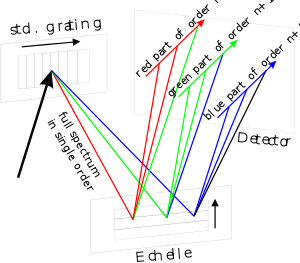
\includegraphics[width=0.4\linewidth, height=3cm]{Imagenes/300px-Echelle_Principle}}
	\subfigure[Red por transmisión]{	
\includegraphics[width=0.4\linewidth,height=3cm]{Imagenes/DiffGrat}}
	\subfigure[Red de difracción plana]{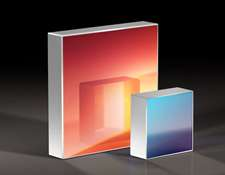
\includegraphics[width=0.4\linewidth,height=3cm]{Imagenes/rejillaPlana}}
	\subfigure[Red de difracción cóncava]{	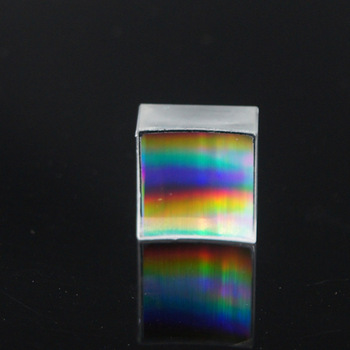
\includegraphics[width=0.4\linewidth,height=3cm]{Imagenes/Spectral-components-Concave-Holographic-Gratings-for-Monochromator}}
	\caption{Redes de difracción, las más comunes son las redes de difracción planas y cóncavas, aún que pueden tener otras formas, como convexa o toroidal \cite{ThorLabs}.}
	\label{fig:redes}
\end{figure}

\subparagraph{Redes de difracción de reflexión.}
La luz incidente en la superficie de estas redes es reflejada a diferentes ángulos, los cuales dependen de la longitud de onda. Con lo cual se puede seleccionar un intervalo espectral. Para calcular este ángulo se usa la ecuación \ref{equa:RedDifra}. Donde \textit{m} es el número de orden, $\lambda$ es la longitud de onda, \textit{d} es la distancia entre líneas contiguas en la red de difracción, $\alpha$ es el ángulo incidente, y $\beta$ el ángulo al que es reflejado, véase figura \ref{fig:reflexion} \cite{Excel2000}.
\begin{equation}
	m\lambda = d(\sin\alpha + \sin\beta)
	\label{equa:RedDifra}
\end{equation}
\begin{figure}[h]
	\centering
	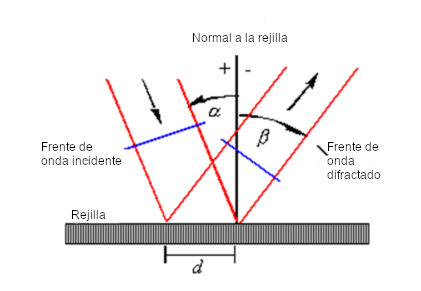
\includegraphics[width=0.6\linewidth]{Imagenes/reflexion}
	\caption{Diagrama de la incidencia y reflexión del haz sobre una red de difracción. $\alpha$ es el ángulo incidente, $\beta$ el reflejado, $d$  es la distancia entre cada línea en la red de difracción, $\lambda$ la longitud de onda. \cite{Excel2000}}
	\label{fig:reflexion}
\end{figure}


\subparagraph{Redes de difracción de transmisión.}
Cuando son de transmisión $\alpha$ es igual a cero ya que la luz incide perpendicular al plano de la red. Sustituyendo en la ecuación \ref{equa:RedDifra}, se simplifica a
\begin{equation}
m\lambda = d\sin\beta
\label{equa:difra}
\end{equation}
\subsubsection{Detector.}
En los espectrómetros actuales frecuentemente el sensor que se utiliza es el CCD, \textit{charge-coupled device}, con este sensor, cada uno de sus pixeles representa una porción del espectro electromagnético. Así al incidir la luz reflejada por la red de difracción se obtiene un espectro inmediato el cual puede ser visualizado en una computadora por medio de un software.

\section{Monocromador}
El monocromador es un dispositivo utilizado para separar la luz en sus diferentes componentes a diferencia de los espectrómetros actuales en los cuales se pueden medir u observar un ancho de banda (todo el espectro visible). En el monocromador, como su nombre lo dice, \textit{mono}, uno, y \textit{chroma} color. Nos dice que a su salida solo obtendremos una longitud de onda, de todas las que esta compuestas la luz.
El monocromador permite hacer barridos, estos barridos no es otra cosa que modificar el
ángulo de incidencia de la luz en la red de difracción. Con lo que se puede ir visualizando a la salida del monocromador, las diferentes longitudes de onda que componen la luz a estudiar. El monocromador, ver figura \ref{fig:1280px-czerny-turnermonochromator}, es similar en configuración a un espectrómetro, la diferencia radica en que después de la rejilla de difracción hay un espejo que se encarga de enfocar las longitudes de onda a una ranura de salida, \textit{slit}, que al igual que el \textit{slit} de entrada, puede variar su apertura, la cual influye también en la resolución espectral del sistema.
\begin{figure}[h]
	\centering
	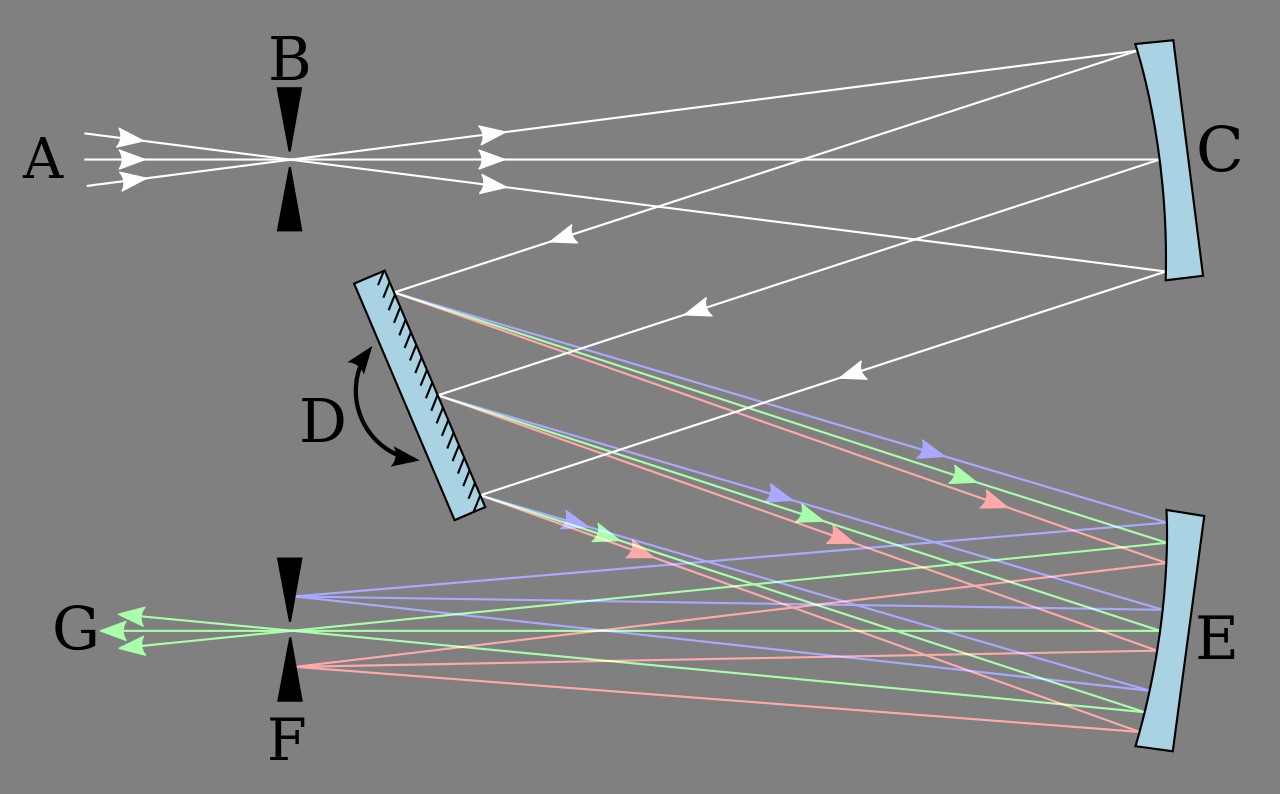
\includegraphics[width=0.4\linewidth]{Imagenes/1280px-Czerny-Turner_Monochromator}
	\caption{Funcionamiento del monocromador. A la salida solo se tiene una longitud de onda. \cite{Czerny-Turney-Conf}}
	\label{fig:1280px-czerny-turnermonochromator}
	
\end{figure}



\section{Tubo fotomultiplicador}
Es un sensor utilizado para poder medir la intensidad luminosa, se le conoce como, PMT, (por sus siglas en inglés, \textit{photomultiplier tube}). Estos sensores, son de alta sensibilidad, son utilizados para medir luz de baja intensidad, o inclusive el conteo de fotones. 
%Los PMts requerían de fuentes de voltajes que iban desde valores de los -1100 volts a los 100 volts, esto para tener diferencias de potenciales en el interior del PMT. Hoy en día existen módulos de PMT que nos permiten ahorrarnos esas fuentes y simplemente conectarlos a $\pm 15$ volts.

Con el monocromador como un sistema para obtener una longitud de onda a la salida y un PMT, como sensor para detectar la intensidad de luminosa a la salida del monocromador, se tienen en principio los elementos para generar espectros.
%tendríamos el principio para construir una relación \textit{intensidad / longitud de onda.} (se modifico.)

\section{Fuentes luminosas.}
Existen varios tipos de fuentes luminosas, como se ha mencionado. Estas pueden tener un espectro de luz continua, de líneas, o bandas. Una fuente luminosa muy importante para este trabajo es la lámpara de mercurio, que posee un espectro de emisión con líneas perfectamente definidas. En la figura \ref{fig:lamparamercurio} se observan las líneas de emisión que tiene la lámpara HG-01 de la empresa Ocean Optics \cite{Excel2000}. Es útil para calibrar nuestro sistema y con ello, garantizar la relación de \textit{intensidad/longitud de onda.}
\begin{figure}[h]
	\centering
	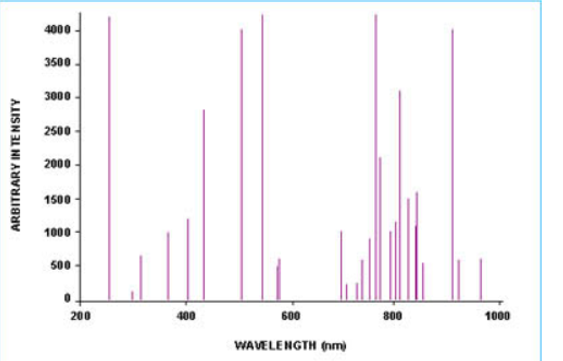
\includegraphics[width=0.7\linewidth]{Imagenes/lamparaMercurio}
	\caption[Espectro de emisión de una lámpara de mercurio a baja presión.]{Espectro de emisión de una lámpara de mercurio a baja presión, la lámpara también emite líneas de argón en longitudes de onda mayores a 600 $nm$. \cite{Excel2000}}
	\label{fig:lamparamercurio}
\end{figure}
\section{Propuesta de sistema.}
Con lo mencionado en este capítulo se entiende que se puede construir un espectrómetro automatizado, con un monocromador, un sensor, un motor a pasos y una tarjeta tanto para controlar y adquirir las señales del sistema; como para visualizar el espectro en una interfaz gráfica. 
\section{Antecedentes.}
Como ejemplos de automatización de espectrómetros, en el año 2016, Jie Liu, Zekun Liu y Zhihong Wang utilizaron un encoder magnético AS5048 para la aplicación en el control de la posición de un motor a DC de un espectrómetro portátil. \cite{JieLiu2016}

Más reciente en el año 2017, E. Galli, A. M. Di Giorgio, M. Focardi, E. Pace y G. Micela desarrollaron un software el cual se encarga del control y procesamiento de información del espectrómetro ARIEL (The Atmospheric Remote-sensing Infrared Exoplanet Large-survey. Se implementó un control sobre el AIRS (ARIEL InfraRed Spectrometer). La unidad de control de instrumentos o ICU, por sus siglas en inglés, fue desarrollado con el propósito de que el sistema a bordo fuera suficientemente capaz de implementar las instrucciones funcionales de control y el procesamiento de los datos siendo esto solo la primera parte para este proyecto. \cite{E.GalliA.M.DiGiorgioM.FocardiE.Pace2017}

En países en desarrollo se busca utilizar las herramientas con que se cuenta y aprovecharlas al máximo. Al tener presupuestos reducidos, muchas veces nos vemos en la necesidad de reutilizar dispositivos con los que ya se cuentan y darles un nuevo uso o una nueva mejora, utilizando tecnología más reciente. Construir un espectrómetro de alta sensibilidad y resolución utilizando un monocromador es la finalidad de este proyecto, y no es la primera vez que se hace este tipo de trabajos, un ejemplo de ello es la automatización de monocromadores modelo MDR-23, realizado en Rusia, para realizar estudios de espectroscopia. \cite{Kraminin2015}

Dentro de la línea de investigación se realizan estudios espectroscópicos de las fuentes luminosas desarrolladas y sobre la interacción de la luz con la materia. Debido al alto costo que conlleva comprar un espectrómetro se decide utilizar los equipos y herramientas con que se cuentan para adaptar un monocromador, que nos servirá para realizar mediciones de espectroscopia.






	\chapter{Marco Teórico.}
En la introducción se habló de forma breve del funcionamiento de los espectrómetros así como de los monocromadores y cómo tienen similitud en su construcción y funcionamiento. La principal diferencia es que con el monocromador solo se obtiene la intensidad de la luz a una longitud de onda a la vez, y los espectrómetros modernos miden la intensidad en un amplio intervalo de longitudes de onda. El monocromador permite realizar barridos, modificando el ángulo de incidencia en la red de difracción, a la salida del monocromador se medirán las intensidades de la luz a las diferentes longitudes de onda. Mientras que el espectrómetro obtiene una imagen instantánea del espectro, en el monocromador se va reconstruyendo longitud de onda a longitud de onda el espectro.

\section{Monocromador.}
El monocromador, al separar la luz en sus diferentes longitudes de onda se puede utilizar para realizar los barridos en intervalos del espectro electromagnético. 
El monocromador a utilizar es un \textit{SpectraPro-275}, de la marca \textit{Action Research Corporation.}
Existen varios tipos de configuraciones para los monocromadores, las más comunes son:

\begin{itemize}
	\item Fastie-Ebert. Ver figura \ref{fig:Configuraciones} (a) consiste en un espejo esférico, y una rejilla de difracción plana. Una sección del espejo se encarga de colimar la luz, y dirigirla a la rejilla, y otra porción se encarga de enfocar la luz difractada hacia el \textit{slit} de salida.
	Es una configuración económica y sencilla, pero tiene ciertos problemas para mantener la calidad de imagen, debido a las aberraciones esférica y de astigmatismo.
	\item  Czerny-Turner. Ver figura \ref{fig:Configuraciones} (b). En este se tienen dos espejos cóncavos, donde el primero se encarga de colimar la luz y el segundo de enfocar la luz difractada, en el \textit{slit} de salida. La geometría de los espejos en esta configuración es flexible, con esto se puede corregir el efecto de coma, las aberraciones esféricas y de astigmatismo. 
\end{itemize} 


\begin{figure}[h]
	\centering
	\subfigure[Fastie-Ebert]{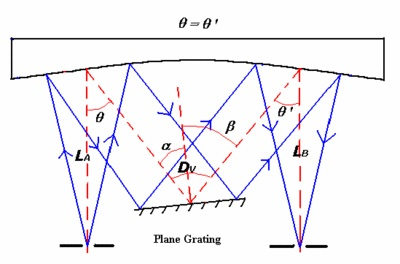
\includegraphics[width=0.7\linewidth]{Imagenes/Fastie-Ebert}}
	\subfigure[Czerny-Turnet]{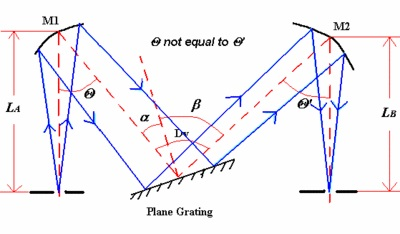
\includegraphics[width=0.7\linewidth]{Imagenes/Czerny-Turner}}
	\label{fig:Configuraciones}
	\caption[Diagramas ópticos de dos tipos de monocromadores de red de difracción.]{Diagramas ópticos de dos tipos de monocromadores de red de difracción. En la configuración (a) solo se tiene un espejo esférico, el cual se encarga de colimar y enfocar la luz, y en la configuración (b) se usan un espejo cóncavo para cada acción. \cite{Gratings2008}} 
	
\end{figure}


\paragraph{Red de difracción.} Es el elemento dispersor del monocromador que se encarga de descomponer la luz en sus diferentes longitudes de onda, dependiendo de las dimensiones de esta así como del periodo de la red o líneas por milímetro. La red, determina el ancho del espectro que pueden trabajar.\\ 
El funcionamiento de las redes de difracción se basa en el fenómeno de difracción y de ahí su nombre. El cual ocurre cuando las ondas pasan a través de una pequeña apertura o un obstáculo perturbando así su propagación, ver figura \ref{fig:difraccion}. En la figura \ref{fig:slit2} se observa un patrón de difracción en una sola rendija.
\begin{figure}[h]
	\centering
	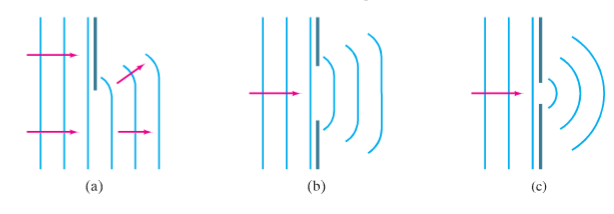
\includegraphics[width=0.9\linewidth]{Imagenes/difraccion}
	\caption{Difracción producida por un obstáculo, por un orificio grande y un orifico pequeño el cual está en el orden de la longitud de onda \cite{Oliver2013a}} %Douglas Cite
	\label{fig:difraccion}
\end{figure}
\begin{figure}[h]
	\centering
	%\subfigure[Patron de difracción ]{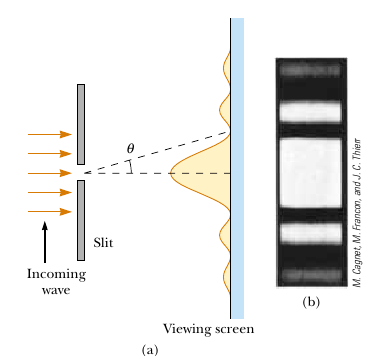
\includegraphics[width=0.48\linewidth,trim={0 10mm 0 0}]{Imagenes/2/slit1}}
	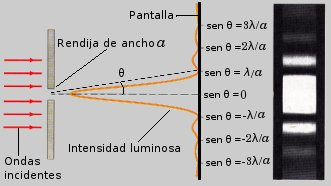
\includegraphics[width=0.7\linewidth]{Imagenes/patronrendijasimple}
	\caption{Fenómeno de difracción en una rendija. ``a'' es el tamaño de la rendija. \cite{longitud01}}
	\label{fig:slit2}
\end{figure} 

En función de la longitud de onda la luz se refleja a un ángulo dado por la ecuación \ref{equa:difra2} (ver ecuación \ref{equa:difra}). Al incidir diferentes longitudes de onda se obtienen distintos valores de $\theta$ dependiendo del orden ($m$). 

\begin{equation}
\sin(\theta) = \frac{m \lambda}{d}
\label{equa:difra2}
\end{equation}

En la figura \ref{fig:difracro} con una longitud de onda menor se observan más ordenes que con una de mayor longitud de onda. 
El fenómeno que sucede en este proceso es el de interferencia. El cual consiste en la superposición de dos o más ondas. Se tiene la superposición constructiva y destructiva, en la primera se fortalecen las ondas y en el otro se contrarrestan. Esto se puede lograr haciendo coincidir dos o más ondas de la misma fuente en un mismo punto, cuando estas han recorrido diferentes caminos.


\begin{figure}
	\centering
	\subfigure[Laser rojo de Helio-Neón $\lambda$=632.8nm]{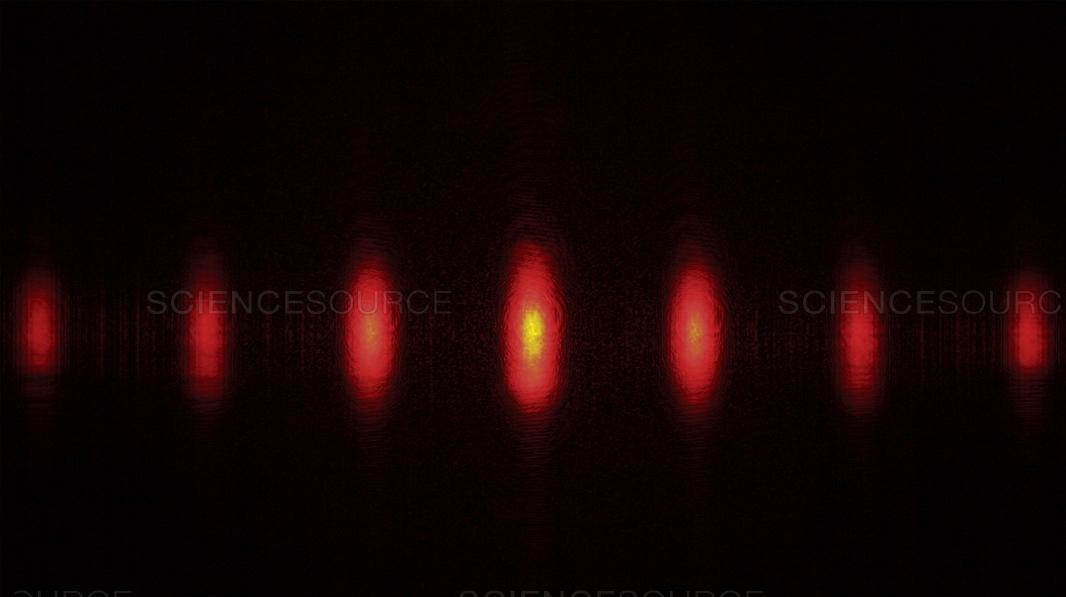
\includegraphics[width=0.48\linewidth, height=4cm]{Imagenes/2/difracRo}}
	\subfigure[Laser verde de Helio-Neón $\lambda$=543.4nm]{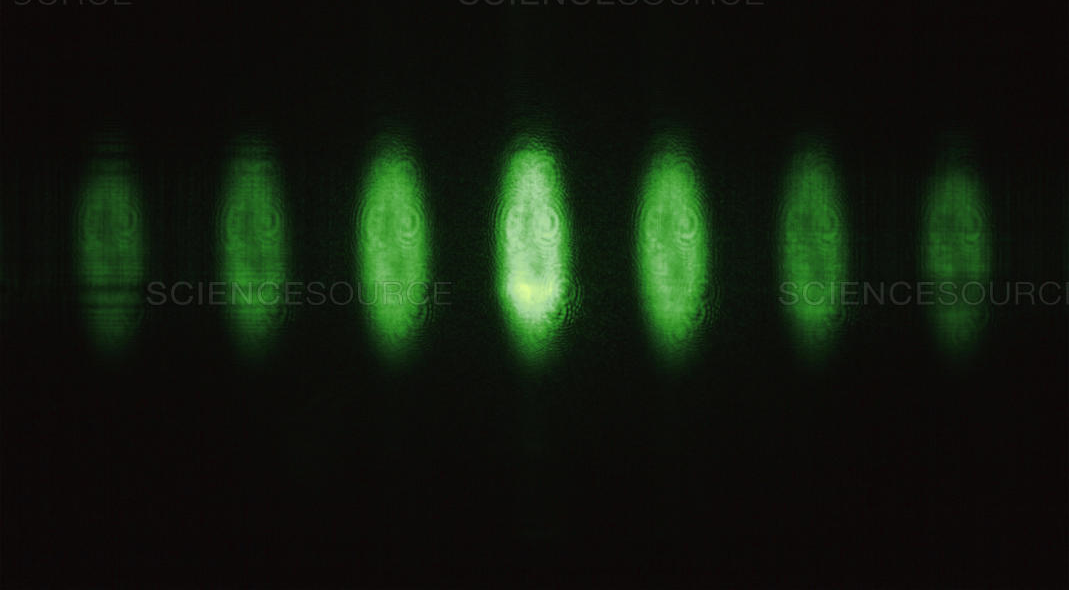
\includegraphics[width=0.48\linewidth,height=4cm]{Imagenes/2/difracGr}}
	\caption[Difracción de la luz con diferentes longitudes de onda.]{Dos láseres de Helio-Neón, rojo $\lambda$=632.8nm y verde $\lambda$=543.4nm. Son difractados en una red de 50 líneas/mm. El espacio entre cada orden de difracción es mayor en relación a la longitud de onda. \cite{laserGR}}
	\label{fig:difracro}
\end{figure}
Al momento de hacer mediciones con los espectrómetros se debe tener cuidado de no confundir los primeros órdenes de las longitudes de onda, con los demás. En la figura \ref{fig:ordenes} se ve como coinciden diferentes longitudes de onda en los mismos ángulos. Esto es de suma importancia cuando se analizan los espectros medidos, para evitar una interpretación incorrecta.

\begin{figure}[h]
	\centering
	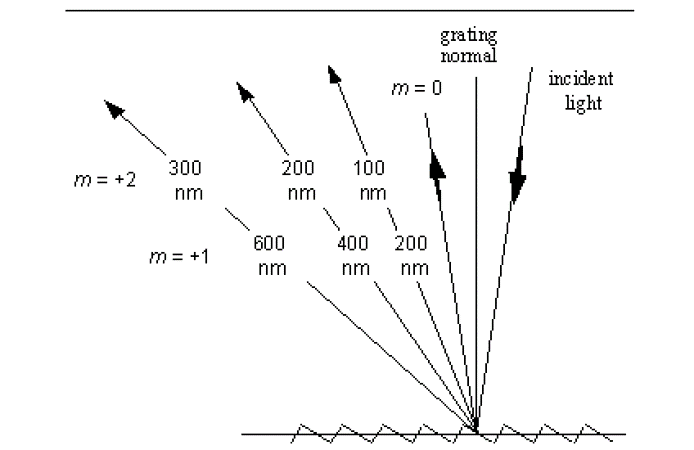
\includegraphics[width=0.7\linewidth]{Imagenes/2/ordenes}
	\caption[Difracción de la luz se aprecia el orden de difracción de diferentes longitudes de onda.]{Luz incidente es difractada y reflejada a diferentes ángulos. Se observa cómo en el mismo ángulo se encuentran dos longitudes de onda diferentes pero de diferente orden. \cite{Palmer2005}}
	\label{fig:ordenes}
\end{figure}


%quitar esto o investigarlo bien. Texto completamente sin sentido.
La eficiencia de difracción es un valor que expresa el grado en que se puede obtener energía de la luz difractada con respecto a la luz incidida.
La eficiencia de difracción es expresada como absoluta o relativa. La primera es el porcentaje de radiación monocromática incidente que es difractada en el orden deseado. La eficiencia de difracción relativa se obtiene dividiendo la eficiencia de difracción absoluta por la reflectancia del material de recubrimiento \cite{Shimadzu}.
Las redes de difracción con alta eficiencia son deseables por muchas razones. Siendo más útiles para medir líneas de baja intensidad. \cite{Palmer2005}
% La segunda por otra parte es la relación de energía difractada en la red, comparada con un espejo recubierto del mismo material que la red
\paragraph{Poder de resolución.} 
Es la capacidad de un espectrómetro para poder diferenciar dos líneas espectrales adyacentes de la misma intensidad. Esta dado por la ecuación \ref{equa:resolucion}. Donde $\Delta\lambda$ es la diferencia entre dos longitudes de onda, m es el orden y N es la cantidad total de líneas en la red de difracción, $N= L\times W_g$, L es la longitud en milímetros de la red, y $W_g$ es la densidad de líneas por milímetro.
\begin{equation}
	R = \frac{\lambda}{\Delta \lambda}
	\label{equa:resolucion}
\end{equation}
\begin{equation}
	R = mN
	\label{equa:resolucion2}
\end{equation}

Tomemos como ejemplo una red de difracción de 1200 líneas/mm con una longitud de 110 mm $R=mN = 1200 \times 110 = 132,000$. De la ecuación \ref{equa:resolucion}. $\Delta\lambda = \frac{R}{\lambda}$. En $\lambda_{500}$, $\Delta\lambda = 0.0038nm$
y en $\lambda_{300}$, $\Delta\lambda = 0.0022nm$. Como se ve, a menores longitudes de onda este poder de resolución es capaz de distinguir entre longitudes de ondas más cercanas, y de forma inversa entre mayor sea la longitud de onda mayor es la distancia entre estas longitudes de onda que podrá resolver \cite{Gratings2008}.

\paragraph{Red de difracción holográfica.} Son recomendadas cuando se quiere trabajar en UV, VIS y NIR. La densidad de líneas debe ser de 1200 líneas/mm o superior. %(hasta los 6000 líneas/mm), Son muy recomendadas para trabajar en UV. 





\subsection{Motor a pasos.}
Este tipo de motores se caracterizan por tener un giro de ángulo específico, al ir cambiando la excitación de sus bobinas. %(borrado todo esto) Al tener un giro tan preciso, son utilizados en sistemas que requieran exactitud, pues el control en motores de AC o DC es más complicado debido a la inercia, así como el control de su velocidad, se desarrollaron los motores a pasos. 
La configuración de los motores a pasos se compone del estator, que es una parte fija, con cavidades, en las cuales se depositan las bobinas del motor, la otra parte es el rotor que es la parte móvil del motor, va montado sobre un eje soportado por dos cojinetes lo que le permite girar libremente, ver fig. \ref{fig:rotorestator}. 

\begin{figure}[h]
	\centering
	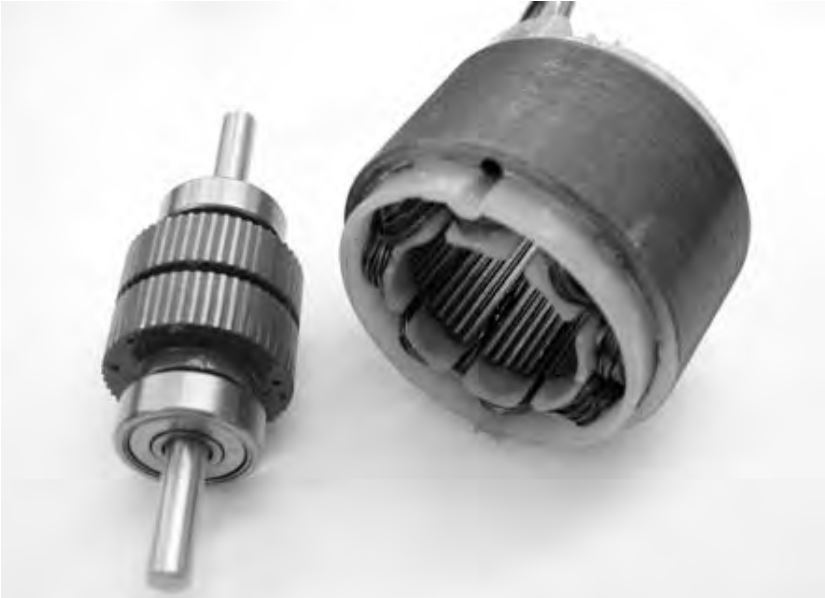
\includegraphics[width=0.7\linewidth]{Imagenes/2/RotorEstator}
	\caption{Esquema de un motor a pasos. Se observan las dos partes principales que le componen. Rotor a la izquierda y estator a la derecha. \cite{Acarnley2002}}
	\label{fig:rotorestator}
\end{figure}
El rotor del motor tiene sus polos N-S, al energizar el estator, este generará sus polos magnéticos N-S, el rotor, buscará el quedar en equilibrio magnético, Norte-Sur y Sur-Norte, lo que provoca que el rotor giré para llegar a este equilibrio. Al cambiar la excitación de las bobinas, los polos N-S creados por el estator, cambiaran, como resultado el rotor volverá a girar, para buscar este punto de equilibrio. De esta forma es como el motor va dando "pasos". En la figura \ref{fig:pasodos} para girar en el sentido de las manecillas del reloj, la bobina energizada (B), debe ser apagada, después se energiza la bobina (C), ocasionando el giro del rotor, para dar un giro desde esta posición, se deben ir encendiendo las bobinas en el siguiente orden C, D, A, B, C, des energizando la última bobina energizada. Para girar en sentido opuesto de las manecillas del reloj simplemente se energizan las bobinas en el orden opuesto, C, B, A, D, C.
Como se aprecia, el control de un motor a pasos es realmente sencillo, y preciso. 
\begin{figure}[h]
	\centering
	\subfigure[primer paso del motor.]{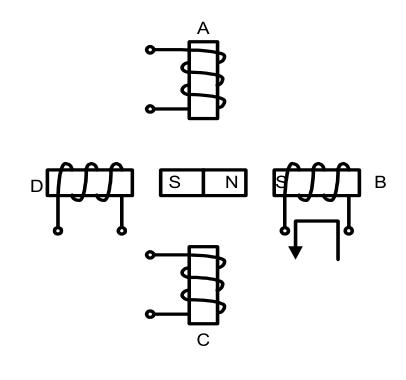
\includegraphics[width=0.4\linewidth]{Imagenes/2/pasoUno}}
	\subfigure[se energiza la bobina C, y el rotor cambia de posición.]{	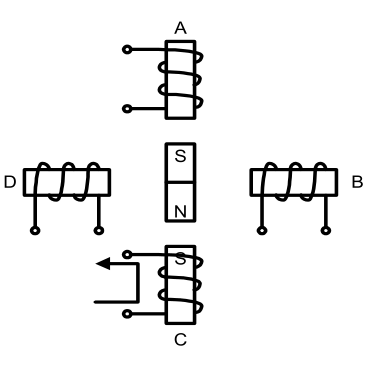
\includegraphics[width=0.4\linewidth]{Imagenes/2/pasoDos}}
	\caption{Giro del rotor en sentido horario.	\cite{BasicStepper}}
	\label{fig:pasodos}
\end{figure}

Los motores a pasos se pueden clasificar en:
\begin{itemize}
	\item Motores de reluctancia variable.
	
	\item Motores de  imán permanente.
	
	\item Motores Híbridos.
	Combinan las características de los dos anteriores donde se tiene un rotor de imán permanente.
\end{itemize}


\paragraph{Control de un motor a pasos.}
El control de motores a pasos se puede realizar de diferentes formas, siguiendo simples secuencias en la alimentación de las bobinas, hay tres formas de mover el motor, paso simple, doble y medio paso. Para el paso simple se energiza solo una bobina a la vez. La secuencia se observa en la tabla \ref{tabla:SecuenciaSimple}. Paso doble consiste en alimentar dos bobinas al mismo tiempo de tal forma que el paso se dé con más fuerza, tabla \ref{tabla:pasoDoble}, pues se generan campos magnéticos en dos bobinas y no sola una. Por último el medio paso, el cual combina el paso simple y doble, logrando así que el motor deba dar el doble de pasos para recorrer la misma distancia angular, tabla \ref{tabla:medioPaso}.
\begin{table}
\centering
\caption{Secuencia para hacer girar un motor a pasos. \cite{BasicStepper}}
\label{tabla:SecuenciaSimple}
\begin{tabular}{|c|c|c|c|c|c|}
	\hline 
	\multicolumn{6}{|c|}{Paso simple motor a pasos} \\ 
	\hline 
	& \hspace{5mm} A \hspace{5mm} & \hspace{5mm} B \hspace{5mm} & \hspace{5mm} C \hspace{5mm} & \hspace{5mm} D \hspace{5mm} & \\ 
	\hline 
	PASO 1  & 1 & 0 & 0 & 0 &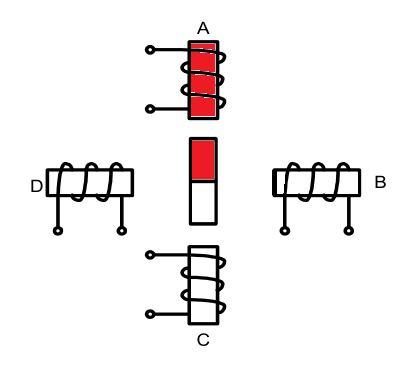
\includegraphics[width=20mm]{Imagenes/2/paso1} \\ 
	\hline 
	PASO 2 & 0 & 1 & 0 & 0 & 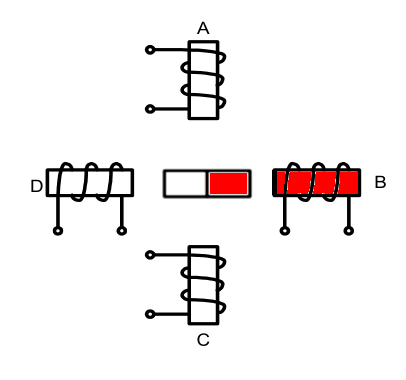
\includegraphics[width=20mm]{Imagenes/2/paso2} \\ 
	\hline 
	PASO 3 & 0 & 0 & 0 & 1 & 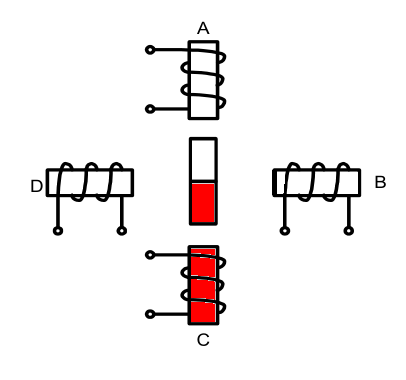
\includegraphics[width=20mm]{Imagenes/2/paso3} \\ 
	\hline 
	PASO 4 & 0 & 0 & 0 & 1 & 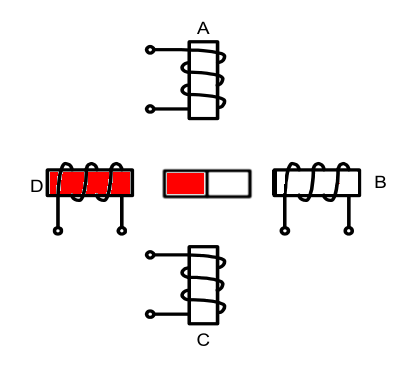
\includegraphics[width=20mm]{Imagenes/2/paso4} \\ 
	\hline 
\end{tabular} 
\end{table}

\begin{table}
	\centering
	\caption{Secuencia de paso "doble", se activan dos bobinas a la vez. \cite{BasicStepper}}
	\label{tabla:pasoDoble}
		\begin{tabular}{|c|c|c|c|c|c|}
			\hline 
			\multicolumn{6}{|c|}{Paso simple motor a pasos} \\ 
			\hline 
			& \hspace{5mm} A \hspace{5mm} & \hspace{5mm} B \hspace{5mm} & \hspace{5mm} C \hspace{5mm} & \hspace{5mm} D \hspace{5mm} & \\ 
			\hline 
			PASO 1  & 1 & 1 & 0 & 0 &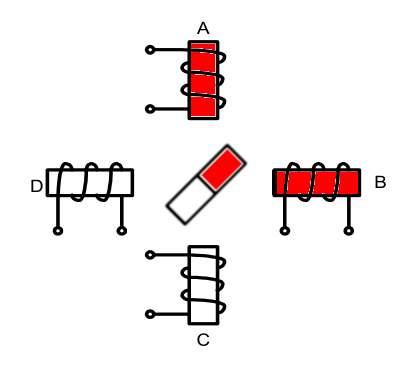
\includegraphics[width=20mm]{Imagenes/2/paso1_5} \\ 
			\hline 
			PASO 2 & 0 & 1 & 1 & 0 & 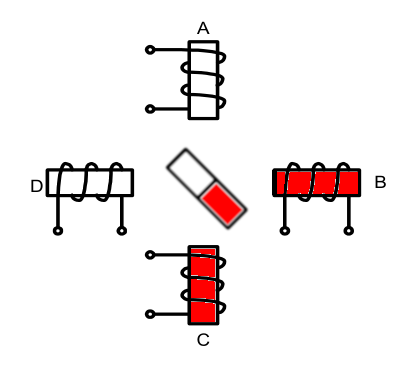
\includegraphics[width=20mm]{Imagenes/2/paso2_5} \\ 
			\hline 
			PASO 3 & 0 & 0 & 1 & 1 & 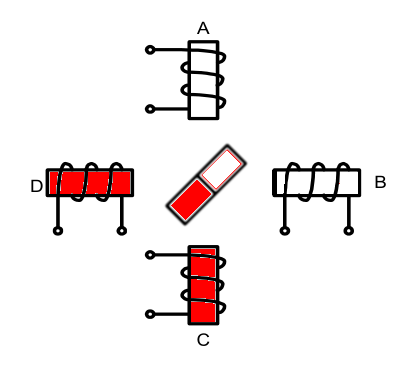
\includegraphics[width=20mm]{Imagenes/2/paso3_5} \\ 
			\hline 
			PASO 4 & 1 & 0 & 0 & 1 & 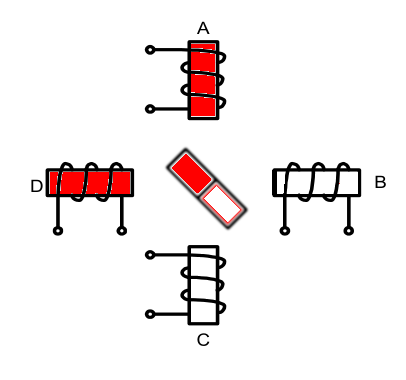
\includegraphics[width=20mm]{Imagenes/2/paso4_5} \\ 
			\hline 
		\end{tabular} 
\end{table}

\begin{table}
	\centering
	\caption{Secuencia para medios pasos, se puede avanzar la mitad de un paso. \cite{BasicStepper}}
	\label{tabla:medioPaso}
	\begin{tabular}{|c|c|c|c|c|p{2cm}|}
		\hline 
		\multicolumn{6}{|c|}{Medio paso} \\ 
		\hline 
		& \hspace{5mm} A \hspace{5mm} & \hspace{5mm} B \hspace{5mm} & \hspace{5mm} C \hspace{5mm} & \hspace{5mm} D \hspace{5mm} & \\ 
		\hline 
		PASO 1 & 1 & 0 & 0 & 0 & 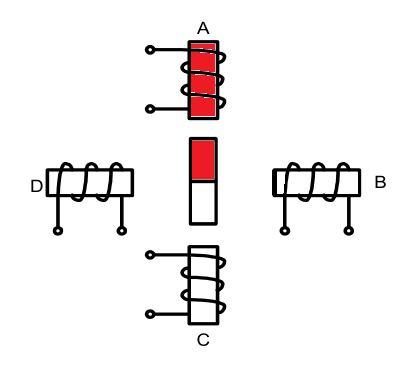
\includegraphics[width=15mm]{Imagenes/2/paso1}  \\ 
		\hline 
		PASO 2 & 1 & 1 & 0 & 0 & 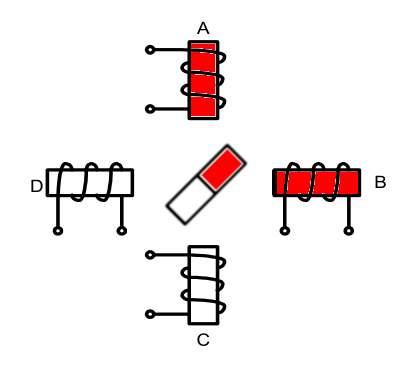
\includegraphics[width=15mm]{Imagenes/2/paso1_5} \\ 
		\hline 
		PASO 3 & 0 & 1 & 0 & 0 & 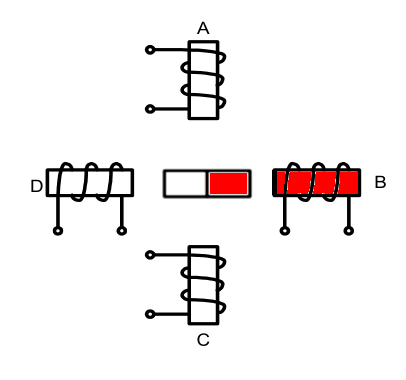
\includegraphics[width=15mm]{Imagenes/2/paso2} \\ 
		\hline 
		PASO 4 & 0 & 1 & 1 & 0 & 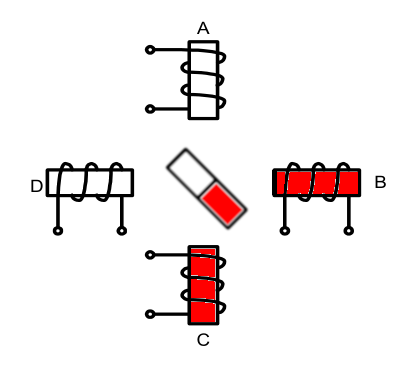
\includegraphics[width=15mm]{Imagenes/2/paso2_5} \\ 
		\hline 
		PASO 5 & 0 & 0 & 1 & 0 & 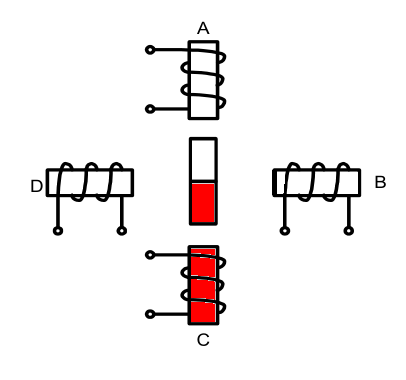
\includegraphics[width=15mm]{Imagenes/2/paso3} \\ 
		\hline 
		PASO 6 & 0 & 0 & 1 & 1 & 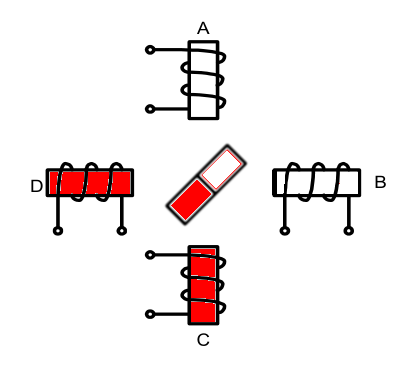
\includegraphics[width=15mm]{Imagenes/2/paso3_5} \\ 
		\hline 
		PASO 7 & 0 & 0 & 0 & 1 & 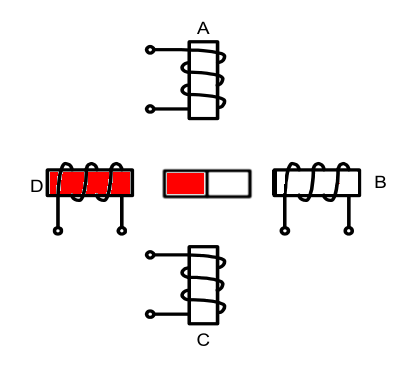
\includegraphics[width=15mm]{Imagenes/2/paso4} \\ 
		\hline 
		PASO 8  & 1 & 0 & 0 & 1 & 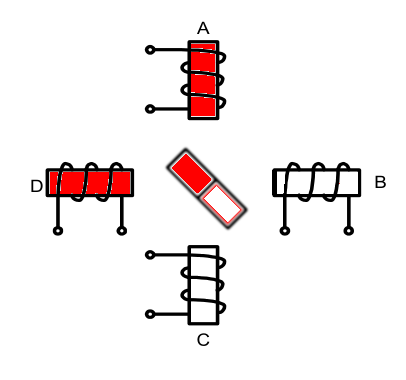
\includegraphics[width=15mm]{Imagenes/2/paso4_5} \\ 
		\hline 
	\end{tabular} 
\end{table}

Con estas secuencias y una etapa de potencia se puede controlar los motores a pasos. Para realizar estas secuencias existen circuitos integrados con 4 pines de entrada y 4 de salida, como el L293D, ver figura \ref{fig:l293}. Este contiene 2 puentes H que tienen como función el ser la etapa de potencia para el motor a pasos, dado que los microcontroladores no tienen la suficiente potencia para hacer girar el motor.
Utilizando este circuito integrado se puede hacer dos tipos de conexiones una a 4 hilos y la otra a 2 hilos. A cuatro hilos, fig. \ref{fig:bipolar-4-fils}, se pueden utilizar los tres tipos de pasos que se mencionaron antes, teniendo más opciones de control, sin embargo, el ocupar 4 pines de salida de un microcontrolador puede ser un inconveniente si es que se quiere mover más de un motor. A dos hilos, fig. \ref{fig:bipolar-2-fils}, solo se puede realizar el paso doble. %Perdemos la posibilidad de utilizar el medio paso que para ciertas aplicaciones puede ser una desventaja.

El control de los motores a pasos no es complicado, sin embargo, hoy en día se tienen otros tipos de circuitos integrados que permiten controlar los motores a pasos, de forma más sencilla. Dentro de estos circuitos integrados, \textit{drivers}, se tienen, el A4988, el DRV8825 y el TB6560, los cuales son muy comunes en las impresoras 3D, pues son de bajo costo y faciles de cambiar. En este trabajo utilizaremos el TB6560.
\begin{figure}[h]
	\centering
	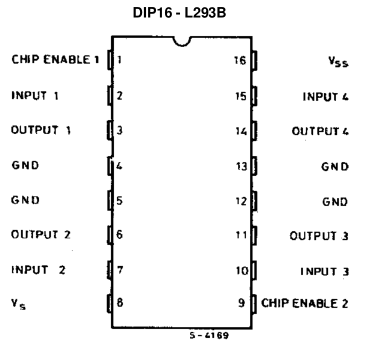
\includegraphics[width=0.4\linewidth]{Imagenes/2/L293}
	\caption[Esquema del circuito integrado L293]{Esquema del circuito integrado L293, se pueden ver los pines de entrada y salida así como el voltaje de alimentación para el circuito. \cite{L2931986}}
	\label{fig:l293}
\end{figure}

\begin{figure}[h]
	\centering
	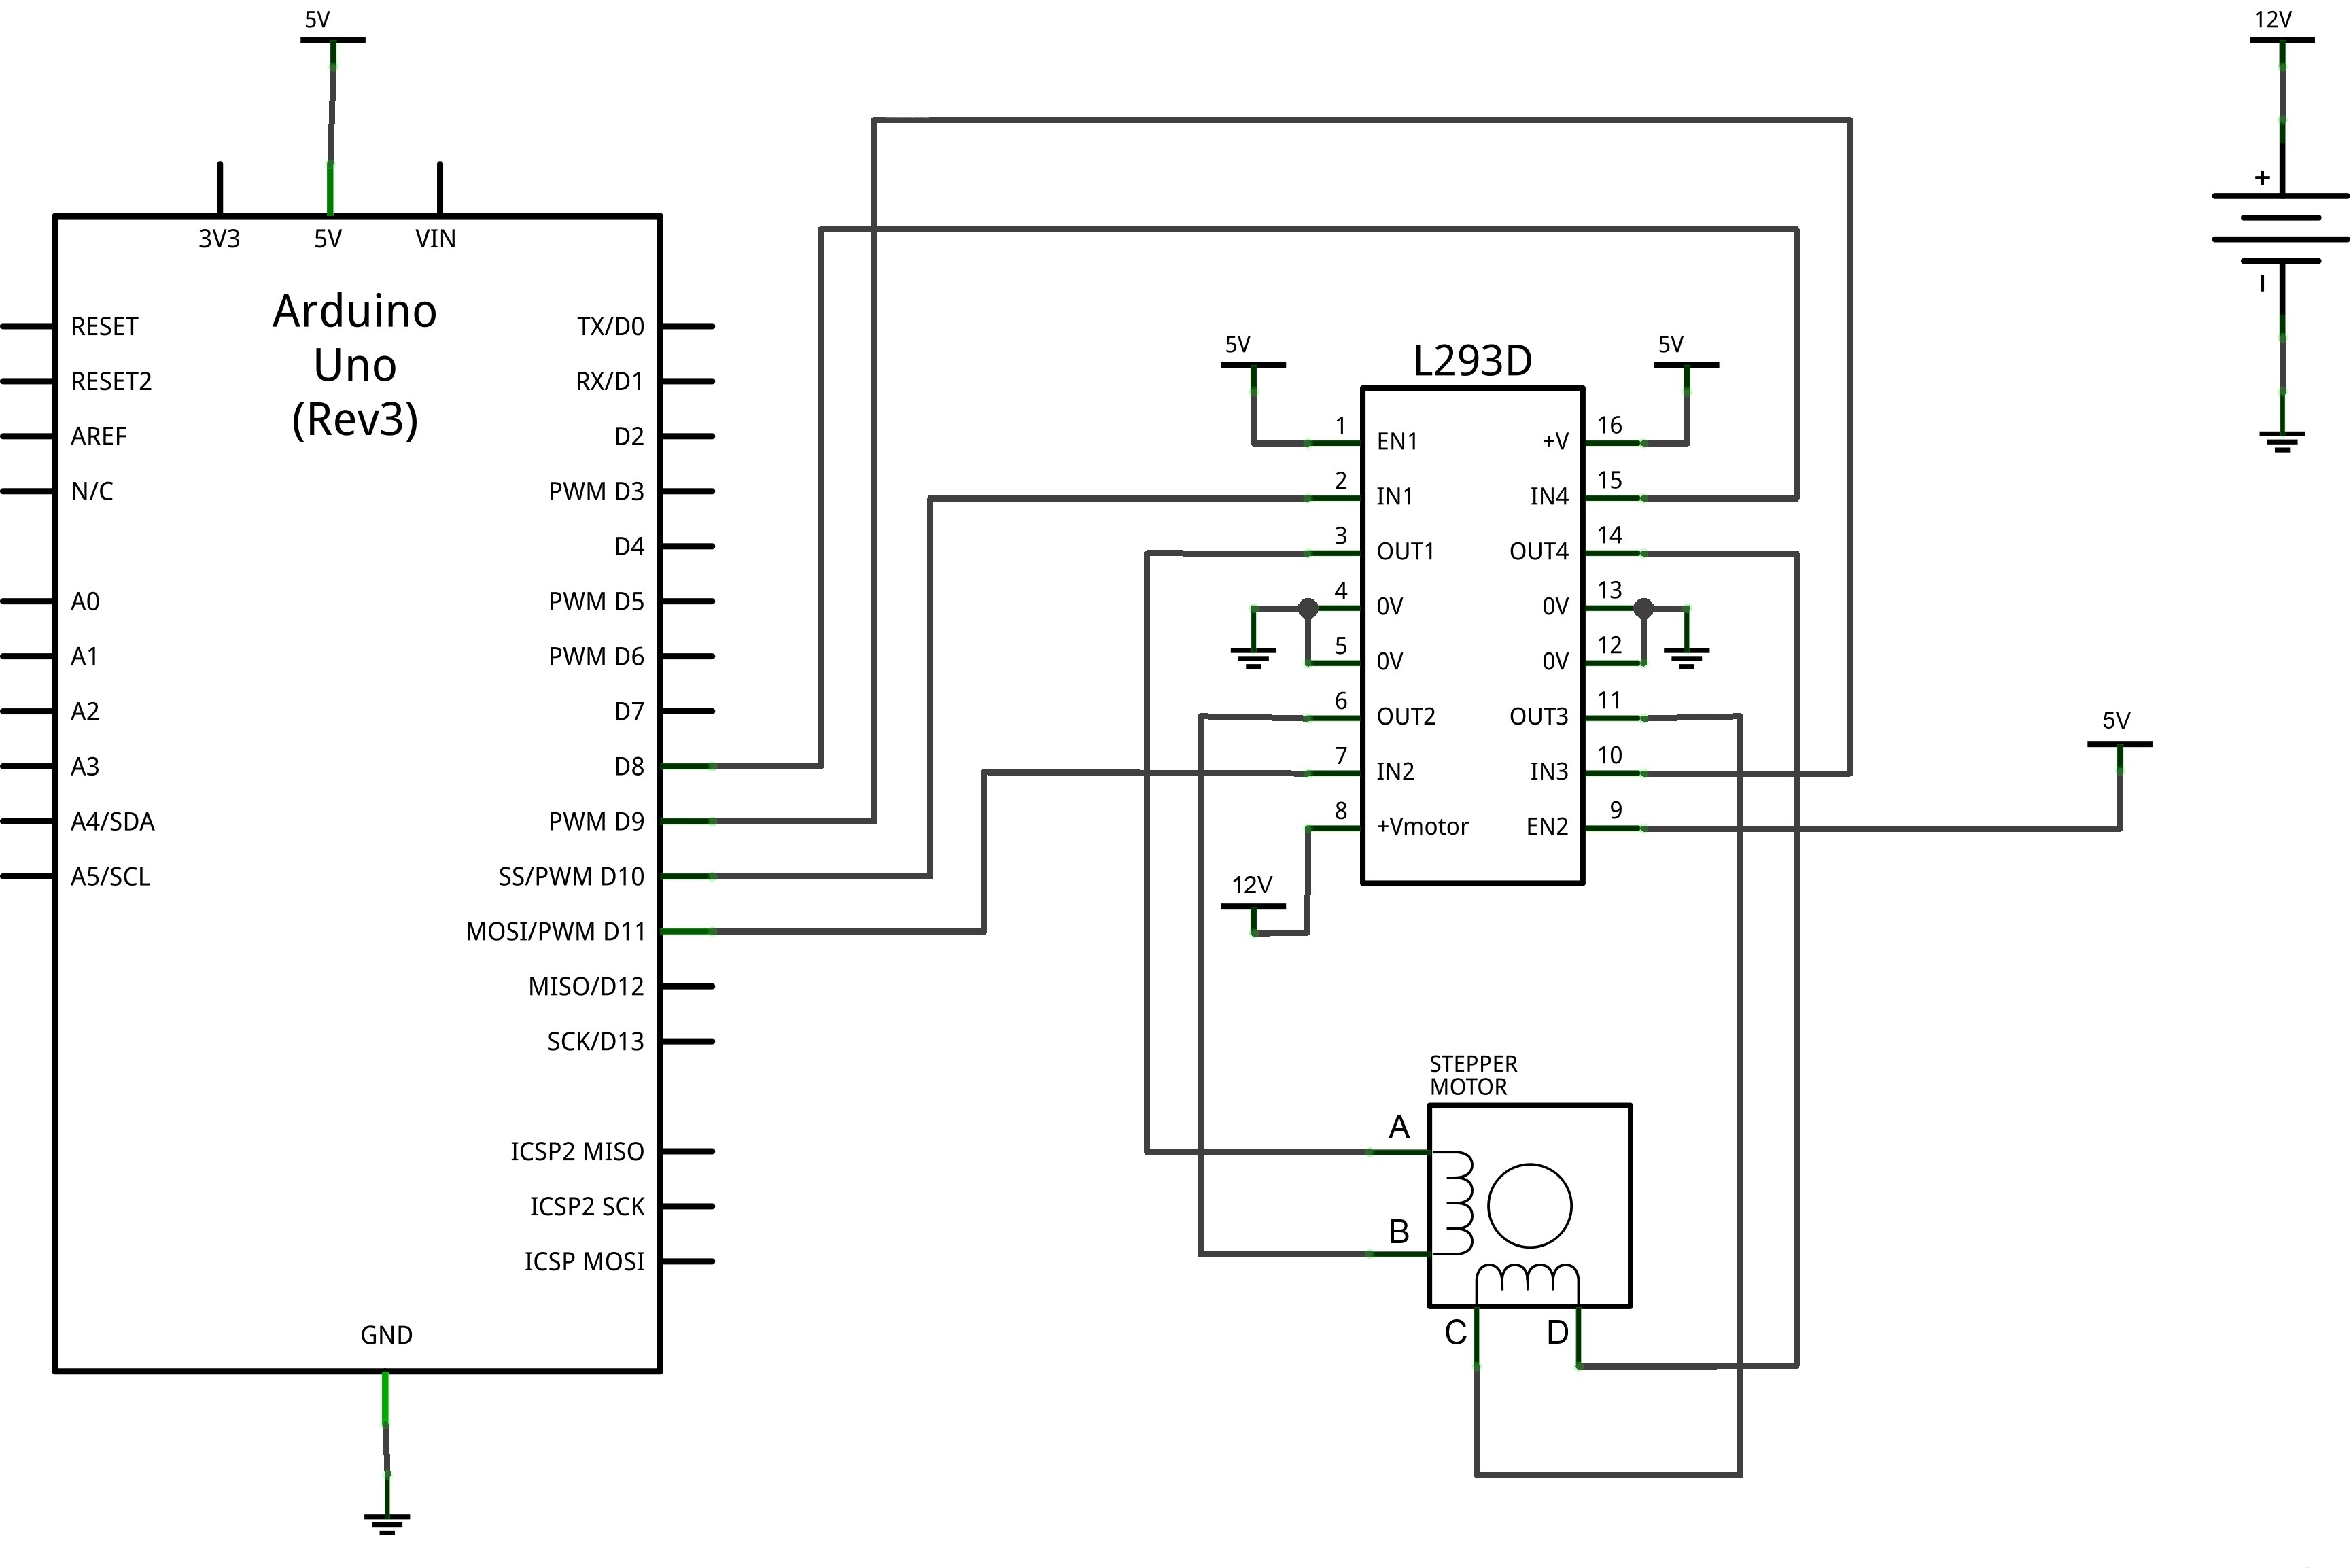
\includegraphics[width=0.7\linewidth]{Imagenes/2/BIPOLAR-4-FILS}
	\caption[Circuito para controlar el motor a pasos con un microcontrolador.]{Circuito para controlar el motor a pasos con un microcontrolador. \cite{Diymakers}}
	\label{fig:bipolar-4-fils}
\end{figure}

\begin{figure}[h]
	\centering
	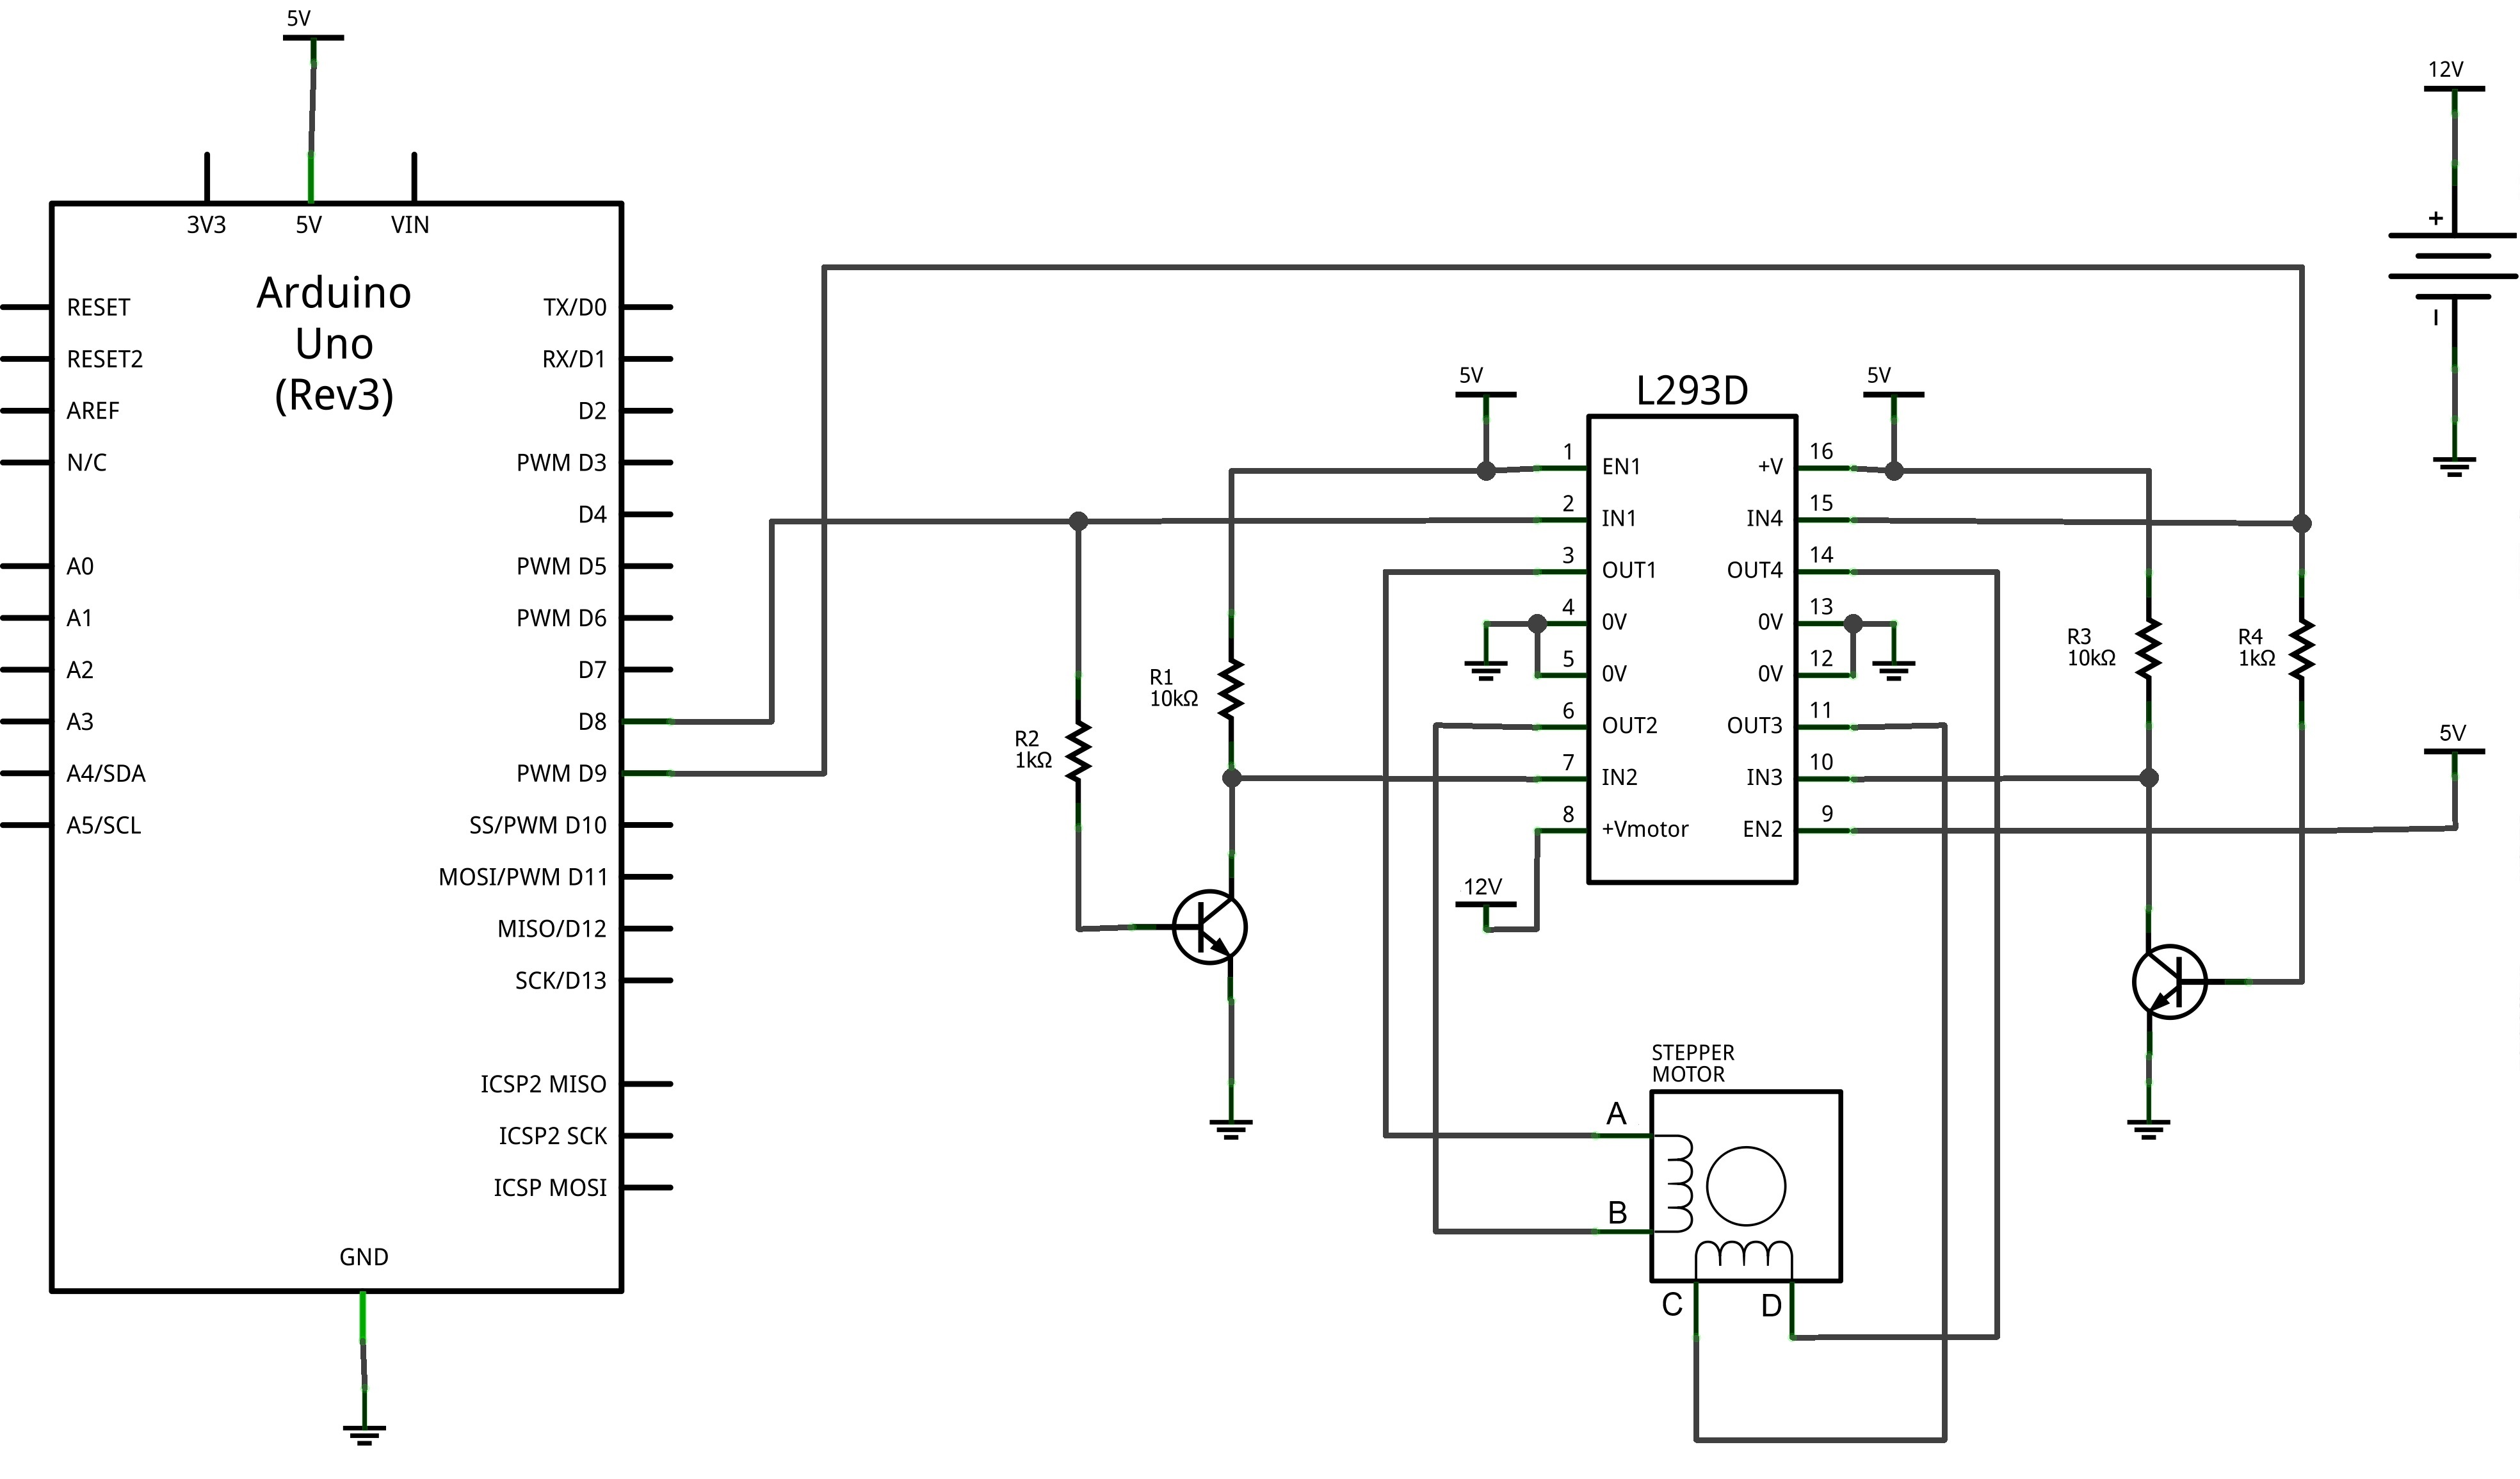
\includegraphics[width=0.8\linewidth]{Imagenes/2/bipolar-2-fils}
	\caption{Circuito utilizando solo dos pines de control. \cite{Diymakers}}
	\label{fig:bipolar-2-fils}
\end{figure}

\paragraph{Driver TB6560.}
 
Es un controlador, \textit{driver}, para motores a paso. El control de los motores a paso, se facilita con este tipo de \textit{drivers}, necesitando solo tres pines de control. Este \textit{driver}, se comercializa ya montado en una tarjeta, esta tarjeta tiene 8 entradas y 4 salidas, así como 9 \textit{switchs}. En la figura \ref{fig:tb6560}, del lado derecho se tienen tres borneras, cada una compuesta de dos pines, de abajo hacia arriba se tienen, (EN-, EN+), (CW-, CW+) y (CLK-, CLK+). Donde EN-, CW-, CLK- son GND, de entrada y las otras tres son los pines de control (EN+, CW+, CLK+), siendo controladas con valores en bajo (0V) y alto (5V, 12V y 24V máximo). A continuación, se explica su función.

\begin{itemize}
	\item EN. Es el \textit{enable}, activación del motor, si este tiene un pulso en alto (5V) el motor estará desenergizado o inhabilitado.
	\item CW. Con esta entrada se controla la dirección del motor. En bajo (0V) el motor girara en sentido horario, y en alto (5V), antihorario.
	\item CLK. Se controla la velocidad del motor, cada pulso en alto es un paso del motor.
\end{itemize}

\begin{figure}[h]
	\centering
	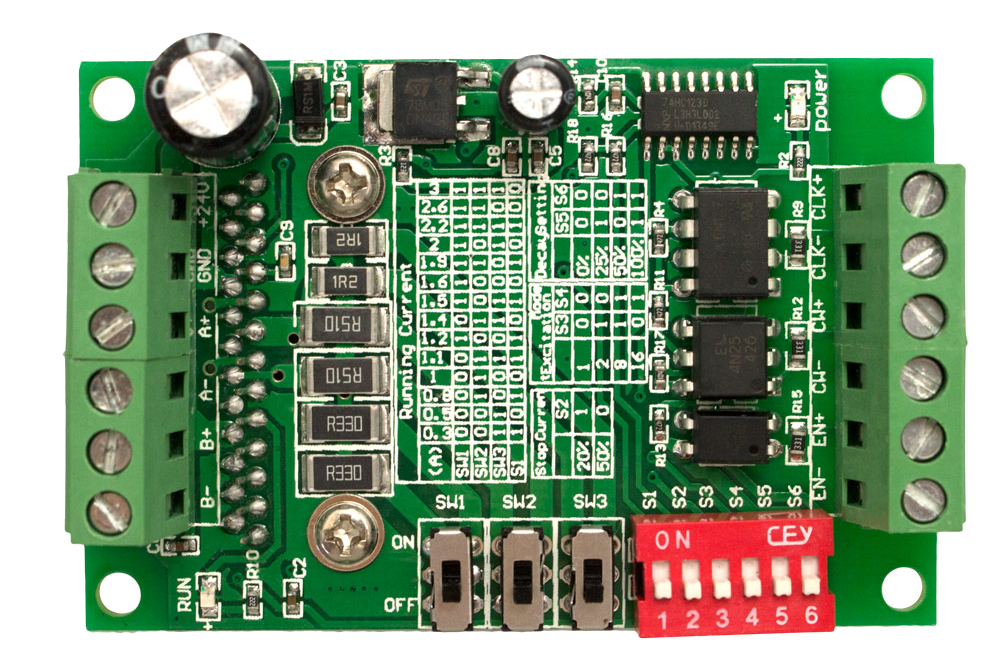
\includegraphics[width=0.7\linewidth]{Imagenes/2/TB6560a}
	\caption{Tarjeta TB6560, control para motores a pasos. \cite{TB6560}}
	\label{fig:tb6560}
\end{figure}
Del lado izquierdo se tienen otras tres borneras de dos pines cada una. De arriba hacia abajo (+24, GND, A+, A-, B+ y B-). 
\begin{itemize}
	\item +24V y GND son las entradas de voltaje para el motor a pasos, el valor máximo es 24V a 3A. 
	\item A+, A-, B+ y B-, son las salidas del \textit{driver}, conectando en estas los cables del motor a pasos, para así controlarlo.
\end{itemize} 

El driver permite limitar la corriente de operación, así como modificar el paso del motor \ref{fig:tmap0051}, logrando  $\frac{1}{16}$ de paso. Por ejemplo, un motor de 200 pasos por vuelta tiene un avance en grados de 1.8 por paso, si se utiliza la configuración de $\frac{1}{16}$ por paso, se tendrán que dar 3200 pasos por vuelta y el avance por paso será de 0.1125° por paso. Se tienen 9 \textit{switchs}:
\begin{itemize}
	\item SW1, SW2, SW3 y S1. Limitan la corriente al motor, en la figura \ref{fig:tmap0051}, en la parte superior se observa la configuración de los \textit{switchs}, para los diferentes valores de corriente.
	\item  S2. Si la corriente aumenta un $20\%$, o $50\%$ sobre el valor establecido, dependiendo de si está en alto o bajo, el motor se detendrá.
	\item  S3 y S4 sirven para variar el paso del motor como se explicó anteriormente. Pasando de paso completo a $\frac{1}{16}$
\end{itemize} 
\begin{figure}[h]
	\centering
	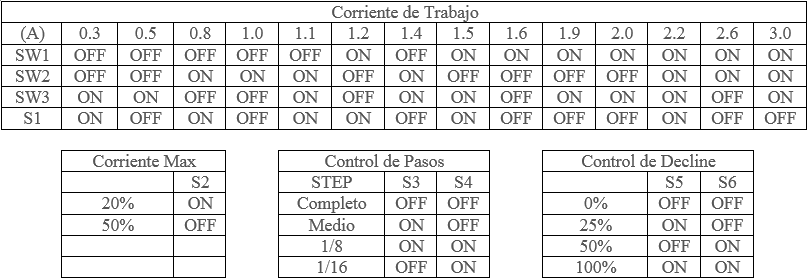
\includegraphics[width=1\linewidth]{Imagenes/2/tmap_0051}
	\caption[Configuración de la tarjeta TB6560]{Configuración de la tarjeta para corriente de trabajo y máxima, control de paso y decline. \cite{TB6560}}
	\label{fig:tmap0051}
\end{figure}

\section{Tubo fotomultiplicador.}
Los tubos fotomultiplicadores son detectores utilizados para medir potencia radiante baja, son especialmente sensibles a la radiación ultravioleta y visible, ver figura \ref{fig:pmte}. EL funcionamiento de los tubos fotomultiplicadores (PMT), se basa en el efecto fotoeléctrico.  
La luz pasa a través de la ventana, \textit{faceplate}, los fotónes inciden en el fotocátodo, y este emite electrones, a los cuales se les llega a llamar fotoelectrones, estos viajan por el interior del PMT.  Los fotoelectrones son acelerados con campos eléctricos y dirigidos al primer dinodo. Con lo cual se desprenden más electrones que los que incidieron, este proceso se repite en cada uno de los siguientes dinodos. Cada dinodo está cargado positivamente 100 voltios más que el anterior. Al llegar al ánodo receptor. Este proceso da como resultado que las pequeñas corrientes generadas por el fotocátodo sean amplificadas millones de veces. Produciendo de $10^5$ a $10^7$ electrones por cada fotón incidente.
Los tubos fotomultiplicadores, son muy sensibles, estando limitados a medir fuentes luminosas de baja potencia, de lo contrario se ocasionarían daños irreversibles en la superficie del fotocátodo.
La figura \ref{fig:pmte} es un esquemático en el que se aprecia cómo está constituido el \textit{PMT}. En la figura \ref{fig:PMT} (a) y (b) se muestran dos tubos fotomultiplicadores, la diferencia entre estos radica en donde incidirá la luz, en el (a) \textit{head-on} es en la parte frontal del \textit{PMT}, y en el (b) \textit{side-on} es el lateral. En la figura \ref{fig:pmtModule} se ven módulos de \textit{PMT}. 
 
 \begin{figure}
	\centering
	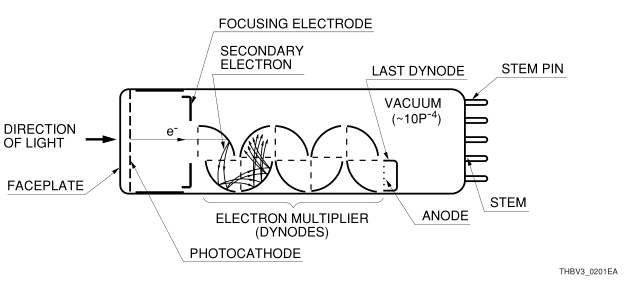
\includegraphics[width=0.9\linewidth]{Imagenes/2/PMT}
	\caption[Esquema de un tubo fotomultiplicador.]{Esquema de un tubo fotomultiplicador.\cite{Hamamatsu2006}}
	\label{fig:pmte}
\end{figure}

Los tubos fotomultiplicadores requerían de una alimentación de alto voltaje partiendo de un voltaje negativo a uno positivo. En cada uno de los dinodos del \textit{PMTs}, se tenía una diferencia de potencial de 100 volts mayor al anterior. De este modo el primer dinodo era alimentado con voltajes de $-1100$ volts hasta llegar al último dinodo el cual tenía ya un voltaje positivo menor a $100$ volts.
%posiblemente se corrija esto xD
Con los módulos de PMT ya solo se debe energizar con un voltaje de $\pm 15$ volts. Para este proyecto se va a trabajar con un módulo de tubo fotomultiplicador de la marca Hamamatsu modelo H8249.

\begin{figure}
	\centering
	\subfigure[PMT \textit{head-on}]{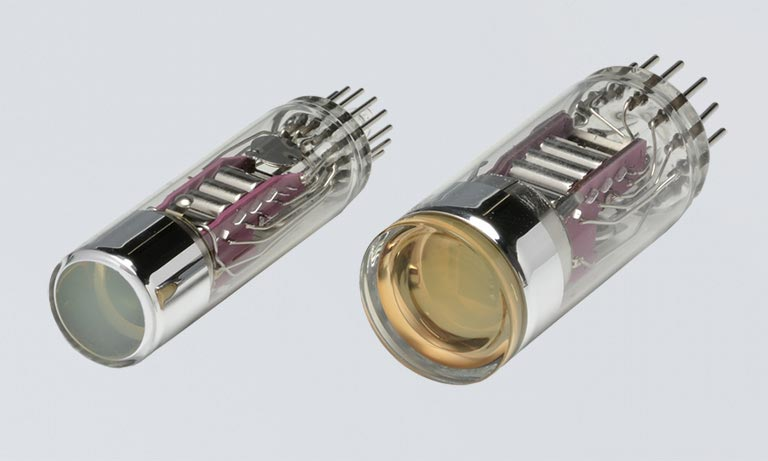
\includegraphics[width=0.4\linewidth]{Imagenes/2/PMThead}}
	\subfigure[PMT \textit{side-on}]{	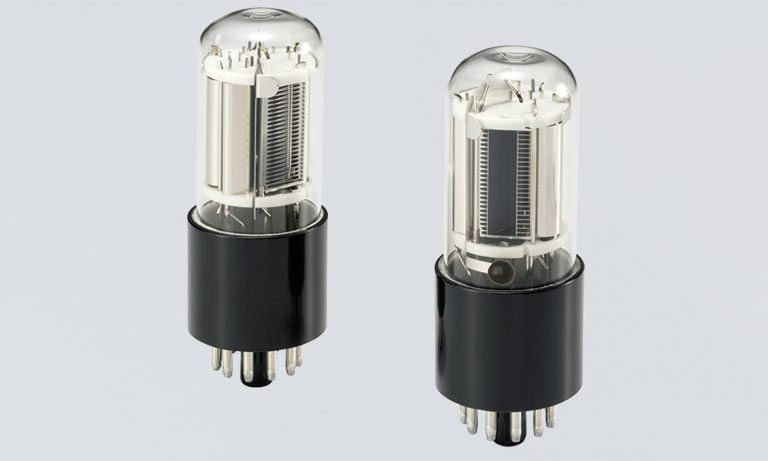
\includegraphics[width=0.4\linewidth]{Imagenes/2/PMTSide-on}}
	\caption[Tubos fotomultiplicadores]{Tubos fotomultiplicadores, de la marca Hamamatsu. \cite{Hamamatsu2007}}
	\label{fig:PMT}
\end{figure}

\begin{figure}
	\centering
	\includegraphics[width=0.7\linewidth]{Imagenes/2/PMTmodule}
	\caption{\textit{PMTs} módulos de la marca Hamamatsu. Están diseñados para diferentes aplicaciones así como para entregar corriente o voltaje a la salida. \cite{Hamamatsu2007}}
	\label{fig:pmtModule}
\end{figure}



\paragraph{Módulo H8249-101.}
La serie H8249 incorpora un \textit{PMT-side-on}, y un circuito de fuente de alto voltaje y una amplificación de bajo ruido. El módulo entrega voltaje a la salida, en su interior cuenta con un circuito de transimpedancia con un factor de conversión de $1V/1\mu A$. El código -101 es el tipo de módulo. Su respuesta espectral va desde los $185nm$ hasta los $900nm$, cubriendo así desde el Ultravioleta medio, luz visible y un poco del infrarrojo cercano.
El módulo cuenta con un ajuste de sensibilidad, figura \ref{fig:sensibilidadajuste}.

\begin{figure}[h]
	\centering
	\includegraphics[width=0.8\linewidth]{Imagenes/2/SensibilidadAjuste}
	\caption[Ajuste de sensibilidad del \textit{PMT módulo H8249}]{Ajuste de sensibilidad del \textit{PMT módulo H8249} puede ser controlado con una fuente de voltaje variable o utilizando una resistencia variable. Con este control se manipula la ganancia que se tendrá en el \textit{PMT}\cite{Hamamatsu2008}}
	\label{fig:sensibilidadajuste}
\end{figure}

 En la figura \ref{fig:sensibilidadajuste} se observa que el módulo se controla con cinco cables, 3 de alimentación, uno de control, y el último un voltaje de referencia, que se puede usar para el control de ganancia, utilizando la configuración de resistencia programable. El voltaje del control de ganancia va desde los 0.2v hasta los 1.2v y la ganancia desde $10^{3}$ hasta $10^{7}$, ver figura \ref{fig:pmtgain}.
 \begin{figure}
 	\centering
 	\includegraphics[width=0.7\linewidth]{Imagenes/2/PMT_GAIN}
 	\caption[Sensibilidad y ganancia H8249]{Sensibilidad del tubo fotomultiplicador (izquierda), voltaje de control apara la ganancia izquierda. \cite{Hamamatsu2008}}
 	\label{fig:pmtgain}
 \end{figure}

\section{Microcontrolador.}
Los microcontroladores son dispositivos programables los cuales cuentan con elementos necesarios para funcionar como una minicomputadora en un solo circuito integrado. %En el interior se encuentran: %el microprocesador, la memoria, los puertos y periféricos. Por ejemplo pensemos en un proyecto para controlar la temperatura, necesitariamos.
%\begin{itemize}
%	\item Leer la temperatura periodicamente y digitalizarla.
%	\item Un control de acuerdo a la temperatura.
%	\item mostrar la temperatura en un \textit{display} de 3 digitos.
%	\item permirir al usuario ajustar la temperatura.
%	\item Y poder configurar el sistema con una interfaz serial. 
%\end{itemize}
%Usando un microprocesador tendríamos que adquirir todas las partes por separa y armar una PCB. Figura \ref{fig:uprocesador}, Ahora que si solo usamos un microcontrolador, este ya integra varias de estos componentes en su interior, siendo más fácil su uso y su programación, figura \ref{fig:ucontrolador}. Se aprecia no solo el tamaño sino la cantidad de componentes es menor.
%Por ello es que los microcontroladores son amplimente usados en diferentes aplicaciones las cuales van desde impresoras, hornos de microondas, sistemas de adquisición de datos, controles automáticos, robots.
%\begin{figure}
%	\centering
%	\includegraphics[width=0.7\linewidth]{Imagenes/2/uprocesador}
%	\caption{Tarjeta PCB con un procesador Z80 para 32 pines (I/O), memoria EEPROM, SRAM, \cite{Lipovski2004}}
%	\label{fig:uprocesador}
%\end{figure}
%\begin{figure}
%	\centering
%	\includegraphics[width=0.7\linewidth]{Imagenes/2/ucontrolador}
%	\caption{Microcontrolador ATmega16 comparado con la tarjeta Z80}
%	\label{fig:ucontrolador}
%\end{figure}


\paragraph{Arduino.} 
Es una tarjeta que se ha popularizado en los últimos años por la facilidad de programación, así como la gran cantidad de librerías y de información en Internet. Arduino goza de una gran comunidad que día a día crean, mejoran bibliotecas y dan soporte para una gran cantidad de aplicaciones. Muchos sensores son vendidos como ``módulos'' para esta tarjeta Arduino, contando con librerías y soportes para su comunicación con softwares como MATLAB o LABVIEW. 

Programando este microcontrolador, se puede controlar y adquirir datos para el desarrollo del espectrómetro. La tarjeta Arduino Mega está basada en el microcontrolador ATmega2560, el cual cuenta con 54 pines digitales de entrada/salida, de los cuales 15 pueden ser utilizados como salidas PWM, 16 entradas analógicas, 4 UART, tiene una velocidad de 16Mhz, conexión por USB, así como una terminal ICSP. 


Para el desarrollo del sistema se requieren de.
\begin{itemize}
	\item 3 pines digitales para el control del motor a pasos.
	\item 2 pines para activar y leer un pulso de un encoder.
	\item 3 pines para el control de un potenciómetro digital.
	\item 4 pines para la comunicación SPI, para un ADC externo.
	\item 2 pines que se usan para la comunicación serial.
\end{itemize}
La tarjeta Arduino Uno, tiene los pines suficientes para este proyecto sin embargo para futuras mejoras esta tarjeta ya no serviría, por ello se decidió utilizar el Arduino Mega.

\paragraph{ADC} el ADC por sus siglas en inglés, (\textit{analog to digital converter}), es un convertidor analógico a digital. Su función es adquirir una señal eléctrica proveniente de un sensor, (voltaje o corriente) y convertirlo a una señal digital, bits. 
La resolución del ADC está dada en bits, (8, 10, 12, 16, 24 bits), o lo que es lo mismo 2 elevado a estas potencias dando como valores, (256, 1024, 4096, 65 536, 16 777 216). Mientras más posibles valores tenga el ADC menor será la diferencia en valor de un bit a otro bit. Por ejemplo, teniendo un voltaje máximo de entrada de 5V para todos estos ADCs, al leer un valor de 1.2V se tendrían los valores mostrados en la siguiente tabla \ref{tabla:adcRe}.

\begin{table}[h]
\centering
\caption{Se muestra la resolución de diferentes ADCs, con un voltaje máximo de entrada de 5 volts.}
\label{tabla:adcRe}
\begin{tabular}{|c|c|c|c|}
	\hline 
	\multicolumn{4}{|c|}{Lectura de un voltaje de 1.2V} \\ 
	\hline 
	Resolución (bits) & Valor digital & voltaje leído (v) & Diferencia mínima que puede leer (mV).\\ 
	\hline 
	8  & 61.44 & 1.191 & 19.53 \\ 
	\hline 
	10 & 245.76  & 1.196 & 4.88\\ 
	\hline 
	12	& 983.04 & 1.199 & 1.22 \\ 
	\hline 
	16	& 15728.64 & 1.2 & 0.076 \\ 
	\hline 
	24	& 4026531.81 & 1.2 & 0.0003 \\ 
	\hline 
\end{tabular} 

\end{table}
\paragraph{ADC-externo.}
El ADC del Arduino Mega es de 10 bits, por lo que se buscó utilizar un ADC de mayor resolución, usando el MCP3202, ver figura \ref{fig:mcp3202}. Es un ADC de dos canales de 12 bits, con comunicación SPI, el valor máximo que puede leer es de 7 volts. El funcionamiento de los pines se explica en la tabla \ref{tabla:ADC}

\begin{figure}[h]
	\centering
	\includegraphics[width=0.5\linewidth]{Imagenes/2/MCP3202}
	\caption{ADC MCP3202 dos canales, 12 bits comunicación SPI \cite{MCP3202}}
	\label{fig:mcp3202}
\end{figure}

\begin{table}[h]
	\centering
	\caption{Tabla con las funciones de los pines del ADC MCP3202 \cite{MCP3202}}
\begin{tabular}{|c|c|}
	\hline 
	Nombre del PIN & Función  \\ 
	\hline 
	CS/SHDN & Chip select, se activa el ADC \\ 
	\hline 
	CH0 & Canal analógico 0 \\ 
	\hline 
	CH1 & Canal analógico 1 \\ 
	\hline 
	$V_{SS}$ & GND del ADC \\
	\hline
	$V_{DD}/V_{REF}$ & Alimentación y voltaje de referencia. \\  
	\hline
	CLK & Velocidad de la comunicación  \\ 
	\hline 
	$D_{IN}$ & Serial Datos de entrada \\ 
	\hline 
	$D_{OUT}$ & Serial datos salida \\ 
	\hline 

\end{tabular} 
	\label{tabla:ADC}
\end{table}

\paragraph{Potenciómetro Digital.}
Como se mencionó el \textit{PMT} necesita de un control de entrada de voltaje. Utilizando el voltaje de referencia que el propio \textit{PMT} genera se requiere un potenciómetro digital para poder variar el voltaje de control del tubo fotomultiplicador. 
El potenciómetro digital es un circuito integrado con el cual uno puede ir variando la resistencia, a través de pulsos digitales, (5v y 0v). EL potenciómetro digital que se uso es el X9C103 \cite{X9C102}. El potenciómetro se observa en la figura \ref{fig:potdig}. Tiene 8 pines, su funcionamiento se explica en la tabla \ref{tabla:potpin}. %CS se activa el potenciómetro digital. Si no esta activo no se puede modificar su resistencia. INC al recibir pulsos va dando pasos en el potenciómetro digital modificando la resistencia. U/D determina si se realizará un incremento o disminución en la resistencia. $V_{CC}$ y $V_{SS}$ son la alimentación del circuito integrado, 5V y GND. $V_h/R_h$ y $V_L/R_L$ son equivalentes a las terminales de un potenciómetro mecánico. $V_W$ es la salida resultante del voltaje.
\begin{figure}[h]
	\centering
	\includegraphics[width=0.5\linewidth]{Imagenes/2/potDig}
	\caption{Potenciómetro digital X9C103 \cite{X9C102}}
	\label{fig:potdig}
\end{figure}

\begin{table}[h]
	\centering
	\caption{Descripción de los pines del potenciómetro digital. \cite{X9C102} }
	\resizebox{15cm}{!}{
	\begin{tabular}{|c|c|}
		\hline 
		PIN & Descripción  \\ 
		\hline 
		INC & Incremento cada cambio de voltaje, alto a bajo, modifica la resistencia en un paso, en la dirección dada por el pin  U/D  \\ 
		\hline 
		U/D & UP/DOWN controla la dirección, (subir o bajar) la resistencia del potenciómetro. \\ 
		\hline 
		$V_H$/$R_H$ & Son los pines equivalentes a las terminales potenciómetro mecánico.  \\ 
		\hline 
		Vss & GND del potenciómetro digital. \\ 
		\hline 
		$V_W$ / $R_W$ & Es la terminal de salida del potenciómetro digital, donde veremos las variaciones de voltaje a la salida. \\ 
		\hline 
		$R_L$/ $V_L$ & Es la terminal en bajo, del potenciómetro digital. \\ 
		\hline 
		CS & el dispositivo es seleccionado cuando su entrada de voltaje está en bajo. Además se puede usar para guardar su posición. \\ 
		\hline 
		Vcc & Voltaje positivo de alimentación del potenciómetro \\ 
		\hline 
	\end{tabular} 
	}
	\label{tabla:potpin}
\end{table}

El \textit{PMT} recomienda usar un potenciómetro digital de $10k\Omega$, el X9C103 es de este valor, con 100 pasos para pasar de una resistencia de 0 hasta $10k\Omega$. Esta cantidad de pasos es más que suficiente para el control de voltaje del \textit{PMT.}


\section{Interfaz gráfica.}
La interfaz gráfica, GUI,  en los sistemas es una de las partes más importante, pues es desde donde se manipula el sistema, y se observarán los datos adquiridos. Uno de los softwares más populares para hacer GUI, (del inglés \textit{Graphical User Interface}) es LabVIEW. LabVIEW es un software que ofrece un enfoque de programación gráfico, lo que lo hace más intuitivo para realizar algoritmos, analizar datos y diseñar interfaces gráficas de usuario. Es por estas características, así como la facilidad de comunicación con Arduino, que se decide utilizar este software.
LabVIEW, \textit{Laboratory Virtual Instrument Engineering Workbench} es un software desarrollado por \textit{National Instruments}. Fue desarrollado originalmente para el \textit{Apple Macintosh} en 1986. Su lenguaje gráfico es llamado "lenguaje G". Hoy en día tiene distribución para los  sistemas operativos como Windows, Unix, Linux y macOS. 









	\chapter{Desarrollo del sistema.}
Para el desarrollo de este sistema espectroscópico se utilizarán los componentes mostrados en la figura \ref{fig:esquema}. A continuación, se explica cómo se utiliza cada uno de los componentes que componen al sistema desarrollado.

\begin{figure}[h]
	\centering
	\includegraphics[width=0.98\linewidth]{Imagenes/3/esquema}
	\caption[Esquema donde se muestran los componentes que se usarán para el sistema desarrollado.]{Esquema donde se muestran los componentes que se usan para el sistema desarrollado. El ángulo de la red de difracción dentro del monocromador es modificado por un motor a pasos. El Driver TB6560 controla el motor a pasos. Todo a través de un microcontrolador. La sensibilidad del PMT es cambiada con un potenciómetro digital.}
	\label{fig:esquema}
\end{figure}

\section{Control del monocromador}
El control del monocromador se basa completamente en el control de giro de la red de difracción. Al girar la red se hace un barrido espectral. Este sirve para poder graficar el espectro punto a punto. Desde la parte exterior del monocromador figura \ref{fig:spectrapro}(a) solo se ve el motor a pasos, la apertura, \textit{slit}, para la entrada de la luz a estudiar, y el \textit{slit} de salida, donde se obtiene solo ``una longitud de onda''. El monocromador posee la configuración Czerny-Turner, figura \ref{fig:spectrapro}(b), la base que tiene la red de difracción permite colocar tres redes, con lo cual este sistema podría adaptarse a mediciones en otros intervalos del espectro electromagnético, con solo cambiar a una de estas redes. 
\begin{figure}[h]
	\centering
	\subfigure[Monocromador SpectraPro 275]{\includegraphics[ height=6cm]{Imagenes/3/SpectraPro}}
	\subfigure[Interior del SpectraPro 275]{\includegraphics[height=6cm]{Imagenes/3/SpectraProIn}}
	\caption{Monocromador SpectraPro 275 de la compañía Action Research Corporation. Se observa desde una vista superior su exterior, (izquierda) y su interior (derecha).}
	\label{fig:spectrapro}
\end{figure}

La red de difracción se encuentra montada en una estructura a la cual llamaremos base, está diseñada para poder seleccionar una de tres redes de difracción. En este proyecto solo se utilizará la red de difracción que tiene mayor densidad de líneas por milímetro (2400 líneas/mm). En la figura \ref{fig:basered2} se aprecia cómo esta estructura está en el interior del monocromador.
\begin{figure}[h]
	\centering
	\subfigure[Base para tres redes de difracción]{\includegraphics[height=4.5cm]{Imagenes/3/baseRed}}
	\subfigure[Vista frontal de las redes sobre la base.]{\includegraphics[height=4.5cm]{Imagenes/3/redDifra_in}}
	\caption{Base del monocromador SpectraPro 275, diseñada para colocar 3 diferentes redes de difracción.}
	\label{fig:basered2}
\end{figure}

En la figura \ref{fig:baseredes} se puede ver una rueda dentada que junto con un tornillo sin fin, que se puede ver en la figura \ref{fig:tornillo}, son los encargados de transmitir el giro del motor a pasos a la red de difracción. 
El motor a pasos está conectado al tornillo sin fin, al girar el motor a pasos con la misma distancia angular de $0.9°$ por paso el tornillo sin fin gira transmitiendo un desplazamiento. En la ecuación \ref{equa:tornillo}, $n$ es el número de vueltas, $Z_2$ es la cantidad de dientes en la rueda y $e$ es el número de entradas del tornillo sin fin.  
\begin{equation}
	n_1 e_1 = n_2 Z_2
	\label{equa:tornillo}
\end{equation}
Dado que $e$ siempre será menor que $Z$, este arreglo funciona como un reductor de velocidad.
//
\linebreak

\begin{figure}[h]
	\centering
	\includegraphics[width=0.4\linewidth,trim={0 0 0 20mm}]{Imagenes/3/baseRedes}
	\caption[Fotografía de la base del monocromador con 3 redes de difracción]{Fotografía de la base, se pueden apreciar dos de las redes de difracción con las cuales cuenta. En la parte inferior se ve la rueda dentada sobre el cual está la base.}
	\label{fig:baseredes}
\end{figure} 
\begin{figure}[h]
	\centering
	\subfigure[Tornillo sin fin]{\includegraphics[height=5cm]{Imagenes/3/tornillo}}
	\hspace{10mm}
	\subfigure[base con rueda dentada sobre el tornillo sin fin.]{\includegraphics[height=5cm]{Imagenes/3/tornillo_base}}
	\caption{Redes de difracción sobre la base y a su vez sobre el tornillo sin fin.}
	\label{fig:tornillo}
\end{figure}

\section{Control de la red de difracción.}
El control del motor a pasos se realiza con el driver TB6560. Como se mencionó antes, solo se necesitan de tres pines para su control. Los cuáles serán los pines 2,3 y 4 del Arduino Mega
\begin{itemize}
	\item pin 2 (dire), se encargará de la dirección del motor.
	\item pin 3 (paso), se encarga del paso del motor, (velocidad, y cantidad de pasos.)
	\item pin 4 (sleep), activa o desactiva el \textit{driver} TB6560
\end{itemize}
%Con un simple algoritmo, donde todos los pines 2, 3 y 4 como salidas. 
El siguiente código hace que el motor a pasos de un solo paso en una dirección (sentido horario). Las variables velL y velH, determinan la velocidad del paso. Si se quiere cambiar el giro del motor solo se debe modificar el valor de \textit{dire} a \textit{LOW}. Ejemplo del código para dar un paso.
\begin{center}
	void pasoMotor() \{ \\
	digitalWrite(sleep, LOW);\\ 
	digitalWrite(dire, HIGH);\\
	digitalWrite(paso, HIGH);\\
	delayMicroseconds(velH);\\
	digitalWrite(paso, LOW);\\
	delayMicroseconds(velL);\\
	\}
\end{center}


%Ya que se puede girar la red de difracción se necesita ubicar a esta en un punto inicial. 
El origen o punto cero, estará determinado por un \textit{encoder}. El monocromador contaba ya con uno, para realizar esta misma función. El \textit{encoder o Optical switch}, es un interruptor óptico. El modelo es el OPB992L51
En la figura \ref{fig:encoder}, se describe el significado de cada uno de las letras y números de este encoder. La información proporciona las características de su empaquetado y como energizar el \textit{encoder}.
\begin{figure}[h]
	\centering
	\includegraphics[width=0.8\linewidth]{Imagenes/3/Encoder}
	\caption{Información del \textit{encoder}, la nomenclatura de este indica su funcionamiento \cite{OPB992}}
	\label{fig:encoder}
\end{figure}
El encoder es el OPB992L51 lo que significa:
\begin{itemize}
	\item OPB, OPTEK Assebly
	\item 9, Familia de sensores \textit{Photologic}
	\item 2 \textit{Inverter Totem-Pole} ver figura \ref{fig:OPB}
	\item L \textit{Emitter}, figura \ref{fig:emitter} (a) y (b).
	\item 51 tamaño de la apertura \ref{fig:emitter} (c).
\end{itemize}
Para poner en funcionamiento el \textit{encoder} se energizar el diodo emisor a traves de los cables rojo y negro, el cable negro va al GND del Arduino, al igual que el cable verde. En la figura \ref{fig:OPB} se observa el cableado del \textit{encoder}. El cable rojo va al Arduino a un PIN de salida, PIN 13, que solo se pone en alto cuando se va a usar el \textit{encoder}, mientras busca la posición cero. El cable azul dará la respuesta cuando su valor esté en bajo significará que se ha encontrado la posición cero, se leerá con el PIN 12 del Arduino.

\begin{figure}[h]
	\centering
	\subfigure[diagrama del encoder.]{\includegraphics[height=40mm]{Imagenes/3/Inverter}}
	\subfigure[Color de los cables]{\includegraphics[height=40mm]{Imagenes/3/Cables}}
	\caption{Información del cableado del \textit{encoder}\cite{OPB992}}
	\label{fig:OPB}
	
\end{figure}
\begin{figure}[h]
	\centering
	\subfigure[]{	\includegraphics[height=30mm]{Imagenes/3/Emitter}}
	\subfigure[]{	\includegraphics[height=30mm]{Imagenes/3/Emitter2}}
	\subfigure[Dimensión de apertura del encoder]{	\includegraphics[height=30mm]{Imagenes/3/51}}
	\caption{Dimensiones del encoder. \cite{OPB992}}
	\label{fig:emitter}
\end{figure}
\begin{figure}[h]
	\centering
	\includegraphics[width=0.7\linewidth,height= 7cm]{Imagenes/3/Encoder_01}
	\caption{Posición cero del sistema, el motor gira hasta que encuentre la ranura de la posición cero.}
	\label{fig:encoder01}
\end{figure}

Al iniciar la búsqueda de la posición cero,
se activa el \textit{encoder} y se hace girar el motor en una dirección de forma continua. El motor hará girar la red de difracción. Al encontrar la posición cero, véase figura \ref{fig:encoder01}. el motor avanzará 400 pasos en la dirección opuesta y regresará a buscar la posición cero, para garantizar que realmente sí la encontró.
Con este algoritmo se coloca el motor en su posición inicial. Para activar el motor se usa una interfaz gráfica en la cual se realiza esta acción con botón 1 de la figura \ref{fig:GUI_01} (1). Al presionar \textbf{INICIAR}, se manda una instrucción al Arduino de girar el motor hasta encontrar la posición inicial, el motor girará mientras en el PIN 12 tenga un valor en ``ALTO'' (5V), cuando el valor este en bajo (0V), el motor estará en su posición inicial.

\begin{figure}[h!]
	\centering
	\includegraphics[width=0.8\linewidth, height=10cm]{Imagenes/3/GUI_01}
	\caption{Interfaz gráfica diseñada para inicializar el sistema.}
	\label{fig:GUI_01}
\end{figure}

\section{Calibración.}
\subsection{Lámpara de mercurio.}
Lo siguiente es realizar los barridos en el intervalo del espectro electromagnético. A partir de la posición cero el motor se mueve paso a paso, donde se tendrá el registro de cada paso. El motor hará girar la red de difracción, desde los 0 pasos hasta los 10000 pasos. Con el algoritmo desarrollado se determina cuantos pasos dar, y en qué sentido. Utilizando el \textit{PMT}, se obtiene un valor de voltaje, proporcional a la intensidad de luz. Se tiene una gráfica pasos vs. voltaje(bits). 
Para esta medición el motor dará un paso y se tomará un valor del \textit{PMT} con el ADC del Arduino MEGA, que tiene una resolución de 10 bits. Se envia la información del paso y valor a la interfaz gráfica, para obtener un espectro que se irá formando paso a paso. En la figura \ref{fig:ledqe65} se aprecia la forma del espectro del led amarillo utilizando nuestro sistema. 


Al comparar los espectros obtenidos, figura \ref{fig:ledqe65}, por nuestro sistema y el espectrómetro QE65000. Se aprecia un espectro mejor definido en el QE65000. Para mejorar el espectro medido por nuestro sistema, se realiza la toma de más muestras por paso, y se obtiene un promedio en cada punto. Con un máximo de 99 muestras por paso, ver figura \ref{fig:led99muestras}.
\begin{figure}[h]
	\centering
	\subfigure[Sistema propuesto.]{	\includegraphics[width=0.45\linewidth]{Imagenes/3/10s30khz-02}}
	\subfigure[QE65000]{\includegraphics[width=0.45\linewidth]{Imagenes/3/LEDQE65}}
	\caption{Espectro del LED amarillo medidos con el sistema propuesto (a) y con el QE65000 (b).}
	\label{fig:ledqe65}
\end{figure}

\begin{figure}[h]
	\centering
	\includegraphics[width=0.9\linewidth,height=6cm]{Imagenes/3/LED99Muestras}
	\caption[Espectro de un LED amarillo.]{Captura del espectro de un LED amarillo, tomando 99 muestras por punto.}
	\label{fig:led99muestras}
\end{figure}

La cantidad de muestras que se toma por punto es de suma importancia para obtener un espectro más limpio y sin tantas variaciones punto a punto.
Para la calibración del sistema se utilizan 99 muestras por paso para medir el espectro de la lámpara de mercurio. Esto con el fin de adquirir un espectro lo más limpio posible y obtener la relación paso a longitud de onda. Las líneas de emisión de la lámpara de mercurio a buscar son 12. En la figura \ref{fig:mercuriolineas} se enlistan.

\begin{figure}[h]
	\centering
	\includegraphics[width=0.8\linewidth,height=5cm]{Imagenes/3/Mercuriolineas}
	\caption{Líneas de emisión de la lámpara de Mercurio. Lámpara de Ocean Optics HG-1 Mercury Argón. Imagen tomada de. \cite{Excel2000}}
	\label{fig:mercuriolineas}
\end{figure}

En la figura \ref{fig:hg-04-m99-50pps}, se pueden apreciar 11 líneas de forma fácil más una de ellas es un segundo orden de la primera longitud de onda de mayor intensidad de la lámpara de mercurio ($\lambda_{253}$ línea (1), su segundo orden $\lambda_{507}$ (8)). Esto se demuestra más adelante utilizando un filtro pasa alto para longitudes de onda mayores a 400nm. Entre las líneas 2 y 4 se alcanza a visualizar una tercera línea, figura \ref{fig:hg-04-m99-50pps} . Entre las líneas 1 y 2 se observa otra pequeña línea (x) de la lámpara. Primero se identifican las líneas de emisión principales de la lámpara de mercurio en nuestro espectro. Estas líneas facilitan la obtención de la relación paso longitud de onda.

\begin{figure}[h]
	\centering
	\subfigure[Espectro de la lámpara de mercurio HG-01 de Ocean Optics]{\includegraphics[width=0.48\linewidth,height=50mm]{Imagenes/3/Hg-04-m99-50pps}}
	\subfigure[Acercamiento a las líneas de emisión.]{	\includegraphics[width=0.48\linewidth,height=45mm]{Imagenes/3/mercuriozoom}}
	
	\caption{Espectro medido con el sistema desarrollado, intensidad contra pasos del motor.}
	\label{fig:hg-04-m99-50pps}
\end{figure}

La lámpara de mercurio tiene en realidad más de 12 líneas de emisión, véase figura \ref{fig:emisionhglibro}. Para poder observarlas se requieren de sistemas de alta resolución y sensibilidad \cite{CRC2016}. Para calibrar el sistema se utilizaron 12 líneas de emisión, ver figura \ref{fig:mercuriolineas}.
% En el libro de \textit{CRC Handbook of Chemistry and Physics"}podemos ver todas las líneas de emisión del mercurio, la figura \ref{fig:espectromercurio}, es una tabla sacada de este libro donde se ven las intensidades y las longitudes de onda (en ángstrom \r{A}) del espectro de emisión de la lámpara de mercurio. En números romanos se encuentra el grado de ionización del mercurio, para nosotros es solo (I) el de interés. Esta es la razón de que en el espectro aparezcan más de las líneas de emisión. 
\begin{figure}
	\centering
	\includegraphics[width=0.9\linewidth,height=5cm]{Imagenes/3/emisionHgLibro}
	\caption{Espectro de emisión del mercurio, se aprecian más de 12 líneas de emisión. Se resaltan las 12 líneas que usaremos para calibrar el sistema desarrollado, \cite{CRC2016}.}
	\label{fig:emisionhglibro}
\end{figure}


\subsection{Relación pasos a longitud de onda.}

Se identificaron los  máximos de cada pico dentro de la medición del espectro adquirido por el sistema. Con los datos obtenidos se graficó el espectro utilizando MATLAB, ver figura \ref{fig:ms1-r}(a). Al hacer un acercamiento al espectro de las líneas de emisión, se logran visualizar más líneas, véase figura \ref{fig:ms1-r}(b). 

%\begin{figure}
%	\centering
%	\includegraphics[width=0.7\linewidth,height=4cm]{Imagenes/3/ms1}
%	\caption{Espectro de la lámpara de mercurio}
%	\label{fig:ms1}
%\end{figure}


\begin{figure}[h]
	\centering
	\subfigure[Pondremos atención a ese recuadro.]{	\includegraphics[width=0.45\linewidth,height=4cm]{Imagenes/3/ms1-r}}
	\subfigure[Se observan más líneas de emisión]{	\includegraphics[width=0.45\linewidth,height=4m]{Imagenes/3/ms1-z}}
	\caption{Líneas de emisión del mercurio. Obtenidas por el sistema, su relación es en pasos y no en longitud de onda.)}
	\label{fig:ms1-r}
\end{figure}


%colocar aquí la imagen faltante.

%\newpage

%\begin{figure}[h]!
%	\centering
%	\includegraphics[width=1\linewidth]{Imagenes/3/EspectroMercurio}
%	\caption{Espectro del mercurio, en números romanos esta el grado de ionización. \cite{Water2017}}
%	\label{fig:espectromercurio}
%\end{figure}

Se realizaron 10 mediciones del espectro de la lámpara de mercurio. En cada una se regresó al punto inicial, posición cero. 

%\includepdf[pages={1},scale=1,pagecommand={}]{Imagenes/3/EspectroMercurio.pdf}

En la figura \ref{fig:medi1}(a) se grafica un solo espectro. Al graficar 10 mediciones del mismo espectro para ver la repetitividad del sistema, véase figura \ref{fig:medi1}(b) se aprecia que hay pocas variaciones entre cada medición. En la figura \ref{fig:medi1}(c), se ve solo uno de los picos de emisión. Cada medición del espectro entrega las mismas líneas de emisión. 

\begin{figure}[h]
	\centering
	\subfigure[Espectro de la lámpara de mercurio medido.]{	\includegraphics[width=0.4\linewidth, height=4cm]{Imagenes/3/medi1}}
	%\subfigure[nos enfocamos en una intervalo.]{	\includegraphics[width=0.4\linewidth]{Imagenes/3/medi1-z}}
	%\subfigure[10 mediciones juntas.]{	\includegraphics[width=0.4\linewidth]{Imagenes/3/medi10}}
	\subfigure[gráfica con 10 mediciones del espectro de la lámpara de mercurio.]{	\includegraphics[width=0.4\linewidth, height=4cm]{Imagenes/3/medi10-z}}
	%\subfigure[aún más cerca en la medición.]{	\includegraphics[width=0.4\linewidth]{Imagenes/3/medi10-z2}}
	\subfigure[Se observa la repetitividad a la hora de medir del sistema, nos enfocamos en solo un pico.]{	\includegraphics[width=0.7\linewidth, height=4cm]{Imagenes/3/medi10-p}}
	
	\caption[Espectro de la lámpara de mercurio. Se aprecia la repetitividad del sistema.]{Espectro de la lámpara de mercurio. se grafican varias mediciones de este espectro para poder observar la repetitividad del sistema a la hora de obtener espectros.}
	\label{fig:medi1}
\end{figure}
Se usan estas mediciones del espectro de la lámpara de mercurio para encontrar las 12 líneas de emisión usadas para calibrar el sistema.
Trabajando con los valores de estos espectros y utilizando la función \textbf{findpeaks} de \textbf{MATLAB}, se encuentran una gran cantidad  picos, ver tabla \ref{tabla:picos01}. 
\begin{table}[h]
	\centering
	\caption{Picos encontrados con \textbf{findpeak} en las mediciones}
	\label{tabla:picos01}
\begin{tabular}{|c|c|c|c|c|}
	\hline 
	picos espectro 1 & picos espectro 2 & picos espectro 3 & picos espectro 4 & picos espectro 5 \\ 
	\hline 
	294 & 299 & 315 & 294 & 353 \\ 
	\hline 
	picos espectro 6 & picos espectro 7 & picos espectro 8 & picos espectro 9 & picos espectro 10 \\ 
	\hline 
	353 & 279 & 279 & 347 & 334 \\ 
	\hline 
\end{tabular} 

\end{table}

Para identificar las 12 líneas de interés se hace un suavizado al espectro, con la función \textit{smooth} en \textbf{MATLAB}. Con el suavizado se eliminan variaciones pequeñas que se tienen en la medición. Además, al colocar la condición de solo encontrar picos con una intensidad igual o mayor a las 12 líneas de emisión que se buscan. Utilizando la función \textbf{findpeaks}. \textit{[picos1,pasos1]=findpeaks(s1,'MinPeakHeigh',20)}. El número de picos encontrados es 14 en cada medición. La función proporciona la intensidad del pico (\textit{picos1}), y la posición, (\textit{pasos1}) donde se encuentra cada pico. 
En la figura \ref{fig:picos14}, se observan estos 14 picos.

\begin{figure}[h]
	\centering
	\includegraphics[width=0.7\linewidth, height=4cm]{Imagenes/3/picos14}
	
	\caption[Espectro de emisión de la lámpara de mercurio, espectro en intensidad contra pasos.]{Espectro de emisión de la lámpara de mercurio donde solo se grafica la posición y la intensidad de los 14 picos encontrados.}
	\label{fig:picos14}
\end{figure}

Con esta información se intenta encontrar cuánto varía un espectro del otro. En la figura \ref{fig:pasoserror} se puede apreciar la diferencia más grande en el paso, en el que se encuentra el pico es de 5 y de 3 la menor. %La desviación estándar del paso se ve en la figura \ref{fig:pasosdes}.

\begin{figure}[h]
	\centering
	\includegraphics[width=0.7\linewidth,height=4cm]{Imagenes/3/pasosError}
	\caption[Diferencias de pasos en los picos encontrados.]{De los 14 picos encontrados se muestra la diferencia entre el paso en el que se encuentra cada pico. El máximo es de 5 pasos de diferencia y siendo 3 pasos lo normal.}
	\label{fig:pasoserror}
\end{figure}

 
%\begin{figure}[h]
%	\centering
%	\includegraphics[width=0.8\linewidth,height=4cm]{Imagenes/3/pasosDes}
%	\caption{Desviación estándar de los pasos en los 14 picos encontrados.}
%	\label{fig:pasosdes}
%\end{figure}

La repetitividad del sistema es buena. Utilizando el promedio de las mediciones hechas se obtiene la relación paso longitud de onda. Al comparar el espectro medido con el sistema y el que se tiene en la literatura, se visualizan líneas de emisión  figura \ref{fig:espectroCompa}.
Para corroborar que varias de las líneas de emisión son de segundo orden se utilizó un filtro que deja pasar longitudes de onda mayores a 415nm. En la figura \ref{fig:hgfiltro} se aprecia como hay líneas de emisión que desaparecen al colocar el filtro. Con esta información se identifican las 12 líneas de emisión para la calibración.
\begin{figure}[h!]
	\centering
	\subfigure[Espectro del Hg 12 líneas (no todas se ven en la gráfica.)]{	\includegraphics[width=0.45\linewidth, height=4cm]{Imagenes/3/espectroHgnor}}
	\subfigure[Espectro del Hg medido 14 líneas]{	\includegraphics[width=0.45\linewidth, height=4cm]{Imagenes/3/espectroHgSistema}}
	\caption{Diferencia visible en la medición del espectro de la lámpara de mercurio. Hay dos líneas que no coinciden que se decide eliminar.}
	\label{fig:espectroCompa}
\end{figure}
\begin{figure}[h!]
	\centering
	\includegraphics[width=0.7\linewidth, height=5cm]{Imagenes/3/HgFiltro}
	\caption[Espectro de la lámpara de mercurio con y sin filtro, intensidad contra pasos.]{Espectro de la lámpara de mercurio con y sin filtro, intensidad contra número de pasos. Se aprecia como la mayoría de las líneas desaparecen. Se prevé estas son menores a 415nm, y de las líneas de mayor longitud de onda solo desaparecen dos.}
	\label{fig:hgfiltro}
\end{figure}


%\begin{figure}
%	\centering
%	\subfigure[Espectro del Hg 12 líneas]{	\includegraphics[width=0.4\linewidth]{Imagenes/3/espectroHgnor}}
%	\subfigure[Espectro del Hg medido 12 líneas]{	\includegraphics[width=0.4\linewidth]{Imagenes/3/espectroHgS12}}
%	\caption{Los espectros lucen visualmente muy similares, al quitar 2 de las líneas.}
%	\label{fig:espectroCom}
%\end{figure}

\subsubsection{Curve Fitting Tool.} 
El \textit{curve fitting} es un proceso para construir una función matemática, que se adapte a una serie de datos. Con este ajuste se tiene una interpolación. Lo que permite tener una relación paso a longitud de onda. Para obtener esta función se deben ingresar dos vectores a la herramienta. En la tabla \ref{tabla:pasolamda} se observan los datos que se utilizaron. El vector \textbf{Pasos} contiene los valores de los pasos en el que se encuentra cada pico. El vector \textbf{Lambda} son los valores de las líneas de emisión en nanómetros. La herramienta nos muestra los valores de "\textit{R-square} y \textit{RMSE}" para elegir la función con el mejor ajuste.
La figura \ref{fig:curving} es una captura de pantalla de la herramienta de \textbf{MATLAB}, \textbf{curve fitting tool}. 

\begin{table}[h]
	\caption{Las 12 líneas de emisión de la lámpara de mercurio, en nanómetros y el número de pasos que se encontró para cada una de estas líneas.}
	\label{tabla:pasolamda}
	\vspace{12mm}
	\begin{tabular}{|c|c|c|c|c|c|}
		\hline 
		Longitud de onda & Pasos & Longitud de onda & Pasos & Longitud de onda & Pasos \\ 
		\hline 
		253.652 & 2803 & 334.148 & 4011 & 435.833 & 5625 \\ 
		\hline 
		296.728 & 3442 & 365.015 & 4488 & 546.074 & 7558 \\ 
		\hline 
		302.150 & 3523 & 404.656 & 5116 & 576.96 & 8149 \\ 
		\hline 
		313.155 & 3690 & 407.783 & 5164 & 579.066 & 8190 \\ 
		\hline 
	\end{tabular} 
	
\end{table}

\begin{figure}[h]
	\centering
	\includegraphics[width=1\linewidth,height=9cm]{Imagenes/3/curving}
	\caption{Interfaz de curve fitting tool de MATLAB.}
	\label{fig:curving}
\end{figure}
El coeficiente de determinación o también llamado $R^{2}$ o \textit{R-square}, en inglés. Es un valor que oscila entre 0 y 1. Entre más cerca este a 1 mayor será el ajuste del modelo a la variable que se está buscando. En general este valor es el más importante a la hora de buscar el mejor ajuste. EL RMSE, \textit{root-mean-square error} por sus siglas en inglés, es la raíz del error cuadrático medio, es una medida de uso frecuente de las diferencias entre los valores predichos por un modelo. Es una medida de precisión, para comparar errores de predicción de diferentes modelos. Su valor es siempre positivo y entre más cercano sea a cero menos es el error del ajuste.

En la tabla \ref{tabla:ajustes} se ve que varios ajustes tienen una \textit{$R^{2}$} igual a 1 pero con diferentes RMSE. El ajuste por Fourier con un solo término es el que tiene un RMSE = 0.1112.

 \begin{table} [h]
\centering
\caption{Diferentes ajustes obtenidos con \textit{curve fitting tool}. Varios de estos ajustes tienen una \textit{R-square} = 1. Por lo que se utiliza el siguiente criterio el RMSE. Siendo Fourier el mejor ajuste.}
\label{tabla:ajustes}
\begin{tabular}{|p{30mm}|p{30mm}|p{10mm}|p{12mm}|p{12mm}|p{12mm}|}
	\hline 
	Tipos de ajuste&Núm. de términos & $R^{2}$ & Adj $R^{2}$& RMSE & SSE \\ 
	\hline 
	Exponencial  & 1 & 0.9828 & 0.9811 & 15.5674 & 2423.4 \\ 
	\hline 
	& 2 & 1& 1 & 0.3485 & 0.9716 \\ 
	\hline 
	\textbf{Fourier} & 1 & 1 & 1 & 0.1112 & 0.0990 \\ 
	\hline 
	& 2 & 1 & 1 & 0.1283 & 0.0988 \\ 
	\hline 
	Gaussian & 3 & 1 & 1 & 0.1214 & 0.0442 \\ 	\hline 
	Polynomial & 3 & 1 & 1 & 0.1112 & 0.0989 \\ 
	\hline 
	Suma de senos & 1 & 1 & 1 & 0.3360 & 1.0161 \\ 
	\hline 
	& 3 & 1 & 1 & 0.1041 & 0.0325 \\ 
	\hline 
\end{tabular} 

\end{table}
La suma de senos con tres términos tiene mejores resultados, pero al intentar resolver la ecuación para obtener la relación opuesta, de longitud de onda a paso se obtenía un error en el paso que se calculaba. Por lo anterior se trabaja con el ajuste de Fourier, con el cual no se presentó este problema, usando la ecuación \ref{equa:pasoLambda}.
\begin{equation}
f(x) = a_0 + a_1\cos (x\times w) + b_1 \sin(x \times w)
\label{equa:pasoLambda}
\end{equation}

Donde: \\
$x = pasos\\
a_0 =-23.77\\
a_1 = 76.47 \\  %(8.576, 247.4)
b_1 = 848.2 \\  %(774.8, 1030)
w = 8.441*10^{-5}$\\  %(7.044e-05, 8.994e-05)
Por lo que la ecuación \ref{equa:pasoLambda} se puede escribir como:\\
\begin{equation}
f(x) =-23.77+76.47 \cos(pasos \times8.441\times10^{-5}) +848.2 \sin(pasos \times8.441\times10^{-5})
\label{equa:pasoLambda2}
\end{equation}

En la tabla \ref{tabla:comparaPasoL} se compara el espectro de emisión de la lámpara de mercurio contra la ecuación del ajuste. El error absoluto más grande es de $0.269$nm. En la figura \ref{fig:compararlp}, se aprecia el espectro de la lámpara de mercurio medido con el sistema. Donde la relación ya es intensidad contra longitud de onda. Los asteriscos azules representan dónde deben aparecer las líneas de emisión. En rojo se aprecia el espectro medido.
   
\begin{table}[h]
	\centering 
	\caption{Comparación de la longitud de las líneas de emisión de la lámpara de mercurio y la ecuación obtenida para encontrar la relación de pasos a longitud de onda ($nm$).}
	\label{tabla:comparaPasoL}
	\begin{tabular}{|p{20mm}|p{20mm}|p{20mm}|p{20mm}|p{20mm}|p{20mm}|}
		\hline 
		 lámpara de Hg & Ajuste de paso a $\lambda$ & Diferencia  & lámpara de Hg & Ajuste de paso a $\lambda$ & Diferencia \\ 
		\hline 
		253.652 & 253.7412 & 0.0892 & 404.656 & 404.6091 & 0.0469 \\ 
		\hline 
		296.728 & 296.7452 & 0.0172 &407.783 & 407.7118 & 0.0712 \\ 
		\hline 
		302.15 & 302.1988 & 0.0488 &435.833 & 435.7680 & 0.065 \\ 
		\hline 
		313.155 & 312.9268 & 0.227 & 546.074 & 546.0847 & 0.0107  \\ 
		\hline 
		334.148 & 333.879 & 0.269 & 576.960 & 576.9355 & 0.0245  \\ 
		\hline 
		365.015 & 365.1355 & 0.1205 &  579.066 & 579.0719 & 0.0059\\ 
		\hline 
	\end{tabular} 
\end{table}

\begin{figure}[h!]
	\centering
	\includegraphics[width=0.8\linewidth,height=6cm]{Imagenes/3/compararLP}
	\caption{El espectro de emisión de la lámpara de mercurio, adquirido por nuestro sistema y ajustado con la ecuación, color rojo. El asterisco azul son las 12 líneas del espectro de emisión del mercurio. Se aprecia como coinciden estas 12 líneas con el espectro obtenido con el sistema.}
	\label{fig:compararlp}
\end{figure}
Este ajuste se introduce en la interfaz gráfica. De esta forma mientras se obtienen los datos, se visualiza el espectro medido, expresado en intensidad relativa contra longitud de onda ver figura \ref{fig:labviewmedir}.\\
\begin{figure}[h!]
	\centering
	\includegraphics[width=0.8 \linewidth, height=6cm]{Imagenes/3/LabViewMedir}
	\caption{Espectro de la lámpara de mercurio medido con el sistema. La intensidad está en unidades relativas y la longitud de onda en nanómetros. El sistema ya está calibrado.}
	\label{fig:labviewmedir}
\end{figure}

\subsection{ADC MCP3202.}
%El ADC MCP3202 tiene una mayor resolución de 12 bits. 
En la figura \ref{fig:ledAmari}, se ve a la izquierda el espectro medido con el ADC del Arduino MEGA y a la derecha el ADC externo. 

\begin{figure}[h]
	\centering
	\subfigure[ADC propio del Arduino MEGA 10bits]{	\includegraphics[width=0.48\linewidth,height=4cm]{Imagenes/3/LedAma10B}}
	\subfigure[ADC- MCP3202 de 12 bits]{	\includegraphics[width=0.48\linewidth,height=4cm]{Imagenes/3/LedAmaB12}}
	\caption{Comparación entre el ADC del Arduino MEGA, izquierda y el ADC MCP3202, derecha. Las dos gráficas están normalizadas.}
	\label{fig:ledAmari}
\end{figure}
El ADC MCP3202, es un ADC de 12 bits de resolución, el cual cuenta con comunicación serial SPI. 
Como se ha mencionado Arduino tiene una amplia comunidad, la cual día a día comparte trabajos y mejoras. Dentro de estos ya existen bibliotecas diseñadas para este ADC en específico. Una de ellas fue desarrollada por Souvik Saha \cite{MITadcLinkedIn}, su trabajo está en un repositorio de \textbf{GitHub}, \cite{MITadc} para que cualquier persona pueda usarlo así como en una página web dedicada a compartir bibliotecas, \cite{MITadcArduino}. Esta biblioteca fue ingresada en nuestro algoritmo.

\subsection{Potenciómetro digital.} 
La sensibilidad del \textbf{PMT} puede ser ajustada variando un voltaje de entrada en el módulo del \textbf{PMT}. Este ajuste se puede realizar de dos formas. Utilizando un potenciómetro o una fuente de voltaje variable ver figura \ref{fig:pmtsen}. Para este control se utilizó un potenciómetro digital. Para manipular el voltaje de control desde la interfaz gráfica.

\begin{figure}[h]
	\centering
	\includegraphics[width=0.9\linewidth]{Imagenes/3/PMTsen}
	\caption[Sensibilidad del PMT.]{Esquema que muestra cómo modificar la sensibilidad del PMT. Esta varía al cambiar el voltaje de control. Se puede realizar con una fuente variable o utilizando un potenciómetro y usando el voltaje de referencia del PMT. \cite{H8249}}
	\label{fig:pmtsen}
\end{figure}
Se tomaron 10 valores de voltaje en cada paso del potenciómetro para ver cómo se comportaba y las variaciones de voltaje, ver figura \ref{fig:adcp1}(a). La figura \ref{fig:adcp1}(b) es la gráfica de la desviación estándar. Al hacer un acercamiento, véase figura \ref{fig:adcp1}(c), se aprecia que la desviación estándar es muy pequeña. En la figura \ref{fig:adcp1}(d) se observa el valor de las desviaciones estándar en cada paso. Siendo de 10mV el valor más grande de la desviación que es equivalente a un paso del potenciómetro digital. 

\begin{figure}[h!]
	\centering
	\subfigure[Voltaje en cada paso del potenciómetro digital.]{\includegraphics[width=0.48\linewidth,height=40mm]{Imagenes/3/ADCp1}}
%	\subfigure[promedio de 10 valores por paso]{\includegraphics[width=0.48\linewidth,height=4cm]{Imagenes/3/ADCp1p}}
	\subfigure[Gráfica de la desviación estándar.]{\includegraphics[width=0.48\linewidth,height=40mm]{Imagenes/3/ADCpSTD}}
	\subfigure[desviación estándar de cerca. La variación de voltaje es de aproximadamente un paso, 10mV.]{\includegraphics[width=0.48\linewidth,height=40mm]{Imagenes/3/ADCpdifz}}
	\subfigure[Valor de la desviación estándar en cada paso.]{\includegraphics[width=0.48\linewidth,height=40mm]{Imagenes/3/ADCpdif}}
%	\subfigure[Grafica de la desviación estandar promedio de 10 valores por paso.]{\includegraphics[width=0.48\linewidth,height=4cm]{Imagenes/3/ADCpSTDp}}

%	\subfigure[error máximo 2.5mV]{\includegraphics[width=0.48\linewidth,height=4cm]{Imagenes/3/ADCpdifp}}
%	\subfigure[Error en porcentaje (0.91\%)]{\includegraphics[width=0.48\linewidth,height=4cm]{Imagenes/3/ADCpor}}
%	\subfigure[Error máximo 0.21\% ]{\includegraphics[width=0.48\linewidth,height=4cm]{Imagenes/3/ADCporp}}
	\caption[Comportamiento del potenciómetro digital X9C103]{Comportamiento del potenciómetro digital X9C103. Utilizando el voltaje de referencia del módulo de \textbf{PMT}. Se aprecia que la desviación estándar es muy pequeña. Así como las variaciones de voltaje, por lo que el sistema podrá medir de forma correcta.}
	\label{fig:adcp1}
\end{figure}
Al aumentar la sensibilidad del \textbf{PMT} se visualizan más líneas de emisión. Al realizar la medición con 0.2V, ya se aprecia el espectro de la lámpara de mercurio, ver figura \ref{fig:hglamp}(a). Al incrementar el voltaje que controla la sensibilidad del \textbf{PMT} a 0.5V se aprecia como en las líneas de emisión $\lambda$=253.6nm y en su segundo orden $\lambda$=507.2nm, el sistema se satura, véase figura \ref{fig:hglamp}(b).
\begin{figure}[h!]
	%\subfigure[Ganancia a 0.10 volts]{\includegraphics[width=0.48\linewidth,height=4cm]{Imagenes/3/Hg01}}
	\subfigure[Ganancia a 0.20 volts]{\includegraphics[width=0.48\linewidth,height=40mm]{Imagenes/3/Hg02}}
%	\subfigure[Ganancia a 0.30 volts]{\includegraphics[width=0.48\linewidth,height=35mm]{Imagenes/3/Hg03}}
%	\subfigure[Ganancia a 0.40 volts]{\includegraphics[width=0.48\linewidth,height=35mm]{Imagenes/3/Hg04}}
	\subfigure[Ganancia a 0.50 volts]{\includegraphics[width=0.48\linewidth,height=40mm]{Imagenes/3/Hg05}}
	\caption[Espectro de lámpara de mercurio medido con diferentes sensibilidades del \textbf{PMT}]{Espectro de lámpara de mercurio medido con diferentes sensibilidades del \textbf{PMT}. Al ir incrementando la sensibilidad del \textbf{PMT}, aumenta la intensidad captada en cada línea de emisión. Con lo que se logra observar más líneas.}
	\label{fig:hglamp}
\end{figure}
\newpage

\section{Intervalo espectral de trabajo del sistema. }
El PMT tiene un intervalo de sensibilidad que va desde los 180 nm hasta los 900 nm. Como se ve en la figura \ref{fig:respuesta}(a), su pico de sensibilidad está en los 400 nm, y a partir de aquí esta decae, al llegar a los 900 nm ya es mínima. Mientras que la red de difracción va desde los 200nm hasta los 850nm véase figura \ref{fig:respuesta}(b). Su máximo pico de eficiencia se encuentra en los 500nm aproximadamente, de aquí baja.
\begin{figure}[h]
	\centering
	\subfigure[Respuesta espectral del \textbf{PMT}, su pico de sensibilidad está en los 400nm]{\includegraphics[width=0.4\linewidth,height=4cm]{Imagenes/3/pmt_sen}}
	\subfigure[Eficiencia de la red de difracción con 2400 líneas/mm]{\includegraphics[width=0.4\linewidth,height=4cm]{Imagenes/3/redEfi}}
	\caption{Respuesta espectral de la red de difracción y del \textbf{PMT}, se aprecia que ambos empiezan en los 200nm, y llegan hasta los 800nm pero con sensibilidad mucho menos (\textbf{PMT}) \cite{H8249} y menor eficiencia (red de difracción. \cite{reddifrac})  }
	\label{fig:respuesta}
\end{figure}

Estos dos componentes serán los que limitarán el intervalo en el que nuestro sistema puede medir espectros. Se revisó el intervalo en el que puede trabajar el sistema, utilizando una lámpara de Tungsteno-Halógeno, LS-1-CAL de OceanOptics, esta lámpara tiene una espectro de emisión que va desde los 300 hasta los 1050 nm \cite{Manual1000}, figura \ref{fig:lamparathd}. %Esta lámpara será más que suficiente para observar la sensibilidad del sistema a longitudes mayores a 600nm.\\
Al medir la lámpara LS-1-CAL, con el sistema desarrollado se tiene una gráfica con un valor máximo en la longitud de onda de 544.1nm, ver figura \ref{fig:lamparath}. Después de $lambda$=544.1nm la intensidad en el espectro decae hasta los 780nm. Esto se debe tanto a la respuesta espectral del tubo fotomultiplicador como de la red de difracción.
\begin{figure}
	\centering
	\includegraphics[width=1\linewidth,height=6cm]{Imagenes/3/lamparaTH_DPNG}
	\caption{Espectro de la lámpara LS-1-CAL de OceanOptics. Usada para calibrar los espectrómetros en potencia. Su intervalo va desde los 300 nm hasta longitudes de onda mayores a los 1000nm. \cite{Manual1000}}
	\label{fig:lamparathd}
\end{figure}
\begin{figure}
	\centering
	\includegraphics[width=1\linewidth,height=6cm]{Imagenes/3/lamparaTH}
	\caption{Lámpara de tungsteno-halógeno de OceanOptics, LS-1-CAL. Medida con el sistema desarrollado. Se observa que el sistema comienza a decaer en sensibilidad a partir de los 540nm aproximadamente. Al llegar a los 780nm el sistema es incapaz de medir.}
	\label{fig:lamparath}
\end{figure}



	\chapter{Mediciones con el sistema}
Se realizaron mediciones con los diferentes espectrómetros para compararlos con nuestro sistema. El espectro de la lámpara de mercurio fue medido con el espectrómetro HR4000 con dos tiempos de integración diferentes. Se observa la medición con 8ms de tiempo de integración en la figura \ref{fig:hr40004ms}(a) y con 100ms de integración \ref{fig:hr40004ms}(b). Se aprecia como el sistema se satura en varias de las líneas de emisión.
\begin{figure}[h]
	\centering
	\subfigure[HR4000, tiempo de integración 8ms]{	\includegraphics[width=0.9\linewidth, height=5cm]{Imagenes/4/HR4000_4ms}}
	%\subfigure[HR4000 40ms]{	\includegraphics[width=0.6\linewidth]{Imagenes/4/HR4000_40ms}}
	\subfigure[HR4000, tiempo de integración 100ms]{	\includegraphics[width=0.9\linewidth, height=5cm]{Imagenes/4/HR4000_100ms}}
	\caption{Espectro de la lámpara de mercurio medido con el espectrómetro HR4000. Se utilizan dos tiempos de integración diferentes.}
	\label{fig:hr40004ms}
\end{figure}
% figura 1
\\
Se tiene el espectro de la lámpara de mercurio medido con el espectrómetro QE65000, el cual a los 8ms de tiempo de integración (el cual es el valor mínimo que acepta), se visualiza como se satura en ciertas longitudes de onda, ver figura \ref{fig:qe650008mshg}.
\begin{figure}[h!]
	\centering
	\subfigure[Espectro de la lámpara de mercurio con un tiempo de integración de 8ms, mínimo del sistema.]{\includegraphics[width=0.9\linewidth, height=4.5cm]{Imagenes/4/QE65000_8msHg}}
	%\subfigure[QE65000 40ms]{\includegraphics[width=0.6\linewidth]{Imagenes/4/QE65000_8msHg}}
	\subfigure[Espectro de la lámpara de mercurio con un tiempo de integración de 100 ms.]{\includegraphics[width=0.9\linewidth, height=4.5cm]{Imagenes/4/QE65000_100msHg}}
	\caption{Espectro de la lámpara de mercurio adquirido con el espectrómetro QE65000. Se aprecia cómo se satura en una gran cantidad de  líneas.}
	\label{fig:qe650008mshg}
\end{figure}
%figura 2

Con el sistema propuesto todas las mediciones se hacen con los \textit{slits} de entrada y de salida en 10$\mu$m, para tener la mayor resolución.  En la figura \ref{fig:spectra100}, se está usando el máximo de sensibilidad en el PMT.
\begin{figure}[h!]
	\centering
	\includegraphics[width=0.9\linewidth, height=5cm]{Imagenes/4/spectra100}
	\caption{Espectro de la lámpara de mercurio medido con el sistema desarrollado. El monocromador tiene los \textit{slits} de entrada y salida en su menor apertura, 10$\mu$m, y en el máximo de sensibilidad del \textbf{PMT}.}
	\label{fig:spectra100}
\end{figure}
%figura 3
%\newpage
Dentro de las 12 líneas de emisión del espectro de mercurio, que se usaron para calibrar. Hay dos líneas que se encuentran relativamente cerca de 576.96 nm y 579.066 nm. En la figura \ref{fig:lineasdos}(a) se observa como el QE65000 no logra resolver las dos líneas, el HR4000, figura \ref{fig:lineasdos}(b) las resuelve y las presenta con un ancho aproximado de 0.5 nm FWMH. Mientras que el sistema desarrollado logra resolver con mayor facilidad estas mismas líneas y las presenta con un ancho de alrededor de 1nm FWMH véase figura \ref{fig:lineasdos}(c). 

\begin{figure}[h]
	\centering
	\subfigure[Líneas de emisión medidas con el QE65000, tiempo de integración 8ms.]{\includegraphics[width=0.48 \linewidth,height=3cm]{Imagenes/4/picosqe}}
	\subfigure[Líneas de emisión medidas con el HR4000, tiempo de integración 3.8ms]{\includegraphics[width=0.48\linewidth,height=3cm]{Imagenes/4/picoshr}}
	\subfigure[Líneas de emisión medidas con el sistema desarrollado. Slits de entrada y salida a 10 $\mu$m, sensibilidad 0.8v.]{\includegraphics[width=0.8\linewidth,height=4.5cm]{Imagenes/4/picos2}}
	\caption{Dos de las líneas de emisión de la lámpara de mercurio $\lambda$= 576.96nm y 579.066 nm. Se aprecia que el sistema desarrollado resuelve mejor estas dos líneas de emisión.}
	\label{fig:lineasdos}
\end{figure}
%\begin{figure}[h]
%	\centering
%	\includegraphics[width=10cm, height=5cm]{Imagenes/4/picosT}
%	\caption[líneas de emisión de la lámpara de mercurio, (576.96nm y 579.066nm)]{líneas de emisión de la lámpara de mercurio, (576.96nm y 579.066nm), se observan pequeñas diferencias entre los sistemas.}
%	\label{fig:picost}
%\end{figure}

%figura 4

En la figura \ref{fig:lst} se visualizan el espectro de la lámpara de tungsteno-halógeno medido con los espectrómetros QE65000, HR4000 y el sistema desarrollado. Como se puede apreciar los espectros con que se cuentan tienen un intervalo de medición mayor al del sistema desarrollado. 
El sistema desarrollado puede medir hasta los 780nm, donde el valor máximo de lectura está en los 544.6 nm. A partir de los 600nm comienza a decaer de forma rápida su sensibilidad. Aún y cuando  el intervalo que el sistema puede medir es menor tiene mejor resolución que los espectrómetros, HR4000 y QE65000 como se ve en la figura \ref{fig:lineasdos}.

\begin{figure}[h]
	\centering
	\includegraphics[width=0.9\linewidth,height=4.5cm]{Imagenes/4/ls_t}
	\caption[Espectro de la lámpara LS-1-CAL]{Lámpara LS-1-CAL, medida con los espectrómetros, HR4000 (verde) y QE65000 (azul), y el sistema desarrollado (rojo). Se observa que el sistema tiene un intervalo menor que el de los dos espectrómetros.}
	\label{fig:lst}
\end{figure}

Se midieron diferentes fuentes luminosas. Donde se encuentran pequeñas diferencias entre los espectrómetros. En la figura \ref{fig:uv380t} se visualiza el espectro de un LED ultravioleta de 385nm un corrimiento de 2nm en el pico medico con nuestro sistema y el QE65000. La figura \ref{fig:uv400} es el espectro de un LED violeta, 400nm, hay una gran similitud entre las tres mediciones(a). Con una diferencia de máximo 0.8nm entre los picos máximos (b). Con un LED rojo $\lambda$ = 650nm, se obtienen resultados similares al LED violeta $\lambda$ = 400nm, véase figura \ref{fig:rojot}(a), donde la diferencia mayor es de 0.6nm ver figura \ref{fig:rojot}(b). En el LED rojo de 700nm encontramos ya una diferencia notoria de casi 20nm, ver figura \ref{fig:r700}, entre el sistema aquí desarrollado y los dos espectrómetros de Ocean Opctics. 
\begin{figure}[h]
	\centering
	\includegraphics[width=0.9\linewidth,height=4.5cm]{Imagenes/4/uv380t}
	\caption[Espectro del LED Ultravioleta 380nm]{Espectro del LED Ultravioleta 380nm. Medido con los dos espectrómetros, (HR4000 y QE65000) y el sistema desarrollado. La gráfica se encuentra normalizada.}
	\label{fig:uv380t}
\end{figure}

\begin{figure}[h]
	\centering
	\subfigure[Espectro del LED violeta, 400nm]{\includegraphics[width=0.48\linewidth, height=3.5cm]{Imagenes/4/UV400}}
	\subfigure[Acercamiento a los máximos.]{\includegraphics[width=0.48\linewidth,height=3.5cm]{Imagenes/4/UV400m}}
	
	\caption[LED violeta $\lambda$= 400nm]{LED violeta $\lambda$=400nm, medido con los espectrómetros HR4000(verde), QE65000(azul) y el sistema (rojo). Los tres instrumentos obtienen el mismo espectro(a). Las diferencias son tan pequeñas que solo se notan al acercarnos al espectro (b).}
	\label{fig:uv400}
\end{figure}
\begin{figure}[h]
	\centering
	\subfigure[LED rojo $\lambda$]{\includegraphics[width=0.48\linewidth, height=3.5cm]{Imagenes/4/rojot}}
	\subfigure[Acercamiento a los máximos]{\includegraphics[width=0.48\linewidth, height=3.5cm]{Imagenes/4/rojom}}

	\caption[LED rojo $\lambda$ = 650nm]{LED rojo $\lambda$ = 650nm medido con los tres sistemas, al igual que con el LED UV $\lambda$= 400nm, se obtiene espectros muy similares (a). Acercándose se observan las pequeñas diferencias que hay en el pico de cada medición (b).}
	\label{fig:rojot}
\end{figure}
\begin{figure}[h]
	\centering
	\subfigure[Espectro del LED rojo $\lambda$=700nm]{\includegraphics[width=0.8\linewidth,height=4cm]{Imagenes/4/r700}}
	\caption[LED rojo, de longitud de onda 700nm]{LED rojo ($\lambda$=700nm) medido con los tres sistemas. En este espectro es donde se observa una diferencia de casi 20nm entre el espectro medido con el sistema y los dos espectrómetros (HR4000 y QE65000).}
	\label{fig:r700}
\end{figure}
\clearpage
Al graficar el espectro del LED rojo ($\lambda$ = 700nm) sobre la respuesta de los sistemas ante la lámpara LS-1-CAL, vemos que el LED rojo está en una zona donde el sistema tiene una menor respuesta y que esta disminuye conforme aumenta la longitud de onda, figura \ref{fig:ls-rojo}. 

El error no se debe al ajuste que se realizó con \textbf{curve fitting tool}. En la gráfica que se observa en la figura \ref{fig:pasotam} podemos apreciar como al ir avanzando en la longitud de onda el paso es cada vez menor. Sin embargo, vemos que de los 650nm a los 700nm no hay una pérdida que muestre que el pico del LED rojo en 700nm aparezca 20nm antes. Por ello concluimos que debido a la combinación de la sensibilidad del PMT y la eficiencia de la red es que el pico aparece antes de lo esperado. 
\begin{figure}[h]
	\centering
	\includegraphics[width=0.9\linewidth,height=5cm]{Imagenes/4/ls-rojo}
	\caption{Espectro de la lámpara LS-1-CAL y el LED rojo $\lambda$ =700nm.}
	\label{fig:ls-rojo}
\end{figure}
\begin{figure}[h]
	\centering
	\includegraphics[width=0.9\linewidth,height=5cm]{Imagenes/4/pasotam}
	\caption{Longitud de onda que se avanza por paso.}
	\label{fig:pasotam}
\end{figure}

\newpage
\section{Ajuste en forma del espectro unidades relativas.}
La lámpara de LS-1-CAL tiene un intervalo desde los 300nm hasta más de los 1000nm. Como se observa en la figura \ref{fig:lst} el sistema desarrollado comienza a perder sensibilidad a partir de los 540nm. Así mismo se observa una medición incorrecta en el LED rojo de 700nm, ver figura \ref{fig:r700} el cual tiene un corrimiento de casi 20nm obteniendo el pico de emisión en 677.8 nm. 
En la tesis ''DISEÑO DE UN SISTEMA PORTÁTIL DE MEDICIÓN
DE IRRADIANCIA ESPECTRAL SOLAR
UTILIZANDO UN ESPECTRÓMETRO'' se realiza un ajuste de potencia de los espectrómetros QE65000 y HR4000 con la lámpara LS-1-CAL \cite{DeInvestigacion2020}. 

En la figura \ref{fig:ls-s-ds} se observa el espectro de la lámpara de tungsteno-halógeno. En azul es la medición con el sistema desarrollado y en rojo los valores de la lámpara con base en el ''\textit{datasheet}''.

\begin{figure}[h]
	\centering
	\includegraphics[width=0.9\linewidth]{Imagenes/4/LS-S-DS}
	\caption[Espectro de la lámpara LS-1-CAL, \textit{datasheet} (rojo), sistema (azul)]{Espectro de la lámpara LS-1-CAL, \textit{datasheet} (rojo), sistema (azul)}
	\label{fig:ls-s-ds}
\end{figure}

Al realizar diferentes mediciones con el sistema desarrollado, variando la potencia, modificando la distancia de la lámpara LS-1-CAL, se obtuvieron las siguientes gráficas, ver figura \ref{fig:ls-potencia}. Donde en la figura \ref{fig:ls-potencia} (a) se tienen mediciones a diferentes potencias en unidades relativas. En la figura \ref{fig:ls-potencia} (b) se observan las mismas gráficas normalizadas. Se ve que el sistema tiene una linealidad en cuanto a la potencia. Con esta información se realiza un ajuste en forma del espectro.  

En la figura \ref{fig:ajusteenforma} se ve como el ajuste realizado hace coincidir el espectro medido con el del \textit{''datasheet''}. La medición del sistema sigue siendo en unidades relativas corrigiendo la forma del espectro. 

\begin{figure}[t]
	\centering
	\subfigure[Espectro de la lámpara LS-1-CAL en unidades relativas.]{\includegraphics[width=0.4\linewidth, height = 3cm]{Imagenes/4/LS-potencia}}
	\subfigure[Espectro de lámpara LS-1-CAL normalizado.]{\includegraphics[width=0.4\linewidth,height = 3cm]{Imagenes/4/LS-potNor}}
	\caption{Espectro de la lámpara LS-1-CAL en unidades relativas.}
	\label{fig:ls-potencia}
\end{figure}

\begin{figure}[h]
	\centering
	\includegraphics[width=0.8\linewidth]{Imagenes/4/ajusteEnForma}
	\caption[Espectro de la lámpara LS-1-CAL medido con el sistema con ajuste de forma]{Espectro de la lámpara LS-1-CAL medido con el sistema con ajuste de forma. En azul es el espectro obtenido en el datasheet, las cruces rojas son el espectro medido con el sistema desarrollado.}
	\label{fig:ajusteenforma}
\end{figure}

Al utilizar este ajuste de forma en la medición del LED rojo de 700nm se observa que su pico de emisión ya aparece de manera correcta a los 700nm, ver figura \ref{fig:ledrojoa}. Aún que a mayor longitud de onda se tiene que el ajuste ya no es optimo por la baja sensibilidad del sistema desarrollado. 
\begin{figure}[h]
	\centering
	\includegraphics[width=0.8\linewidth,height=5cm]{Imagenes/4/LEDrojoA}
	\caption[Espectro de un LED rojo (700nm) con ajuste de forma.]{Espectro de un LED rojo (700nm) con ajuste de forma. Se observa que el pico del espectro con ajuste (rojo) ya tiene su pico de emisión a los 700nm a diferencia del que se presenta sin ajuste (azul), el cual se presenta en los 680nm aproximadamente.}
	\label{fig:ledrojoa}
\end{figure}

Dado que la lámpara LS-1-CAL tiene un intervalo de emisión de los 300nm en adelante. Este ajuste de forma solo nos sirve en un intervalo de 300nm a 700nm. El sistema desarrollado es capaz de detectar longitudes de onda menores a 300 nm por lo cuál se decide colocar la opción de utilizar o no este ajuste de forma. Al medir espectros de línea de emisión menores a 600nm no es necesario usar el ajuste. Al medir longitudes de ondas superiores a 300 nm se recomienda activar el ajuste de forma.



 

	\specialhead{Conclusiones}
Utilizando un monocromador SpectraPro 275 de la marca Action Research Corporation que se tenía en el laboratorio, un tubo foto multiplicador Hamamatsu, modelo H8249-101 y con un sistema desarrollado para el control de movimiento de un motor a pasos, se construyó un sistema espectrométrico automatizado y el mismo fue debidamente caracterizado.
El sistema es capaz de realizar mediciones dentro de un intervalo de los 250nm hasta los 700 nm, con un paso de 0.067nm que disminuye a 0.042nm. En este intervalo resuelve mejor las líneas espectrales. Como ejemplo tenemos las dos líneas de emisión del mercurio en 576.96nm y 579.066nm dónde se aprecia un FWHM de 0.5nm en el sistema desarrollado. Mientras que el HR4000 es tiene un FWHM de más de 1nm y el QE65000 no logra resolverlas. \\

%La lampara de mercurio y la herramienta de \textbf{curve fitting tool}, fueron de gran utilidad para encontrar una relación paso a longitud de onda. \\
%
%La lampara de tungsteno-halogeno nos ayudo a ver el intervalo en el que se puede medir con el sistema.\\
%
%Los espectros medidos con este sistema servirán para identificar lineas de emisión pero al no tener una calibración en potencia, la forma del espectro no será la correcta, en ciertos intervalos del espectro. \\



	\specialhead{Trabajo futuro.}
La lámpara de tugsteno-halógeno, \textbf{LS-1-CAL}, se utilizo para hacer un ajuste en forma del espectro. Sin embargo como trabajo futuro el sistema podría ser calibrado en unidades absolutas teniendo un ajuste en potencia. \\
%La lámpara de tungsteno-halógeno, \textbf{LS-1-CAL}, puede ser utilizada para hacer una calibración de la respuesta del sistema desarrollado. Esto garantizaría que el sistema pueda medir a longitudes mayores a 650nm con mejor exactitud. \\

Utilizar un ADC de mayor resolución mejoraría la obtención de los espectros. Permitiendo medir variaciones de intensidad más pequeños.\\

Se pueden utilizar las otras redes de difracción con sensores que tengan un intervalo de operación en longitud de onda mayor. Sin embargo, estas redes de difracción nos darían menor resolución. 

	\begin{flushright}
		
\end{flushright}%%%%%%%%%%%%%%%%%%%%%%%%%%%%%%%%%%%%%%%%%%%%%%%%%%%%%%%%%%%%%%%%%%% 
%                                                                 %
%                           BIBLIOGRAPHY                          %
%                                                                 %
%%%%%%%%%%%%%%%%%%%%%%%%%%%%%%%%%%%%%%%%%%%%%%%%%%%%%%%%%%%%%%%%%%% 
 
%This method produces a numbered bibliography where the numbers
%correspond to the \cite commands in the text. See the LaTeX manual.
%
\bibliographystyle{ieeetr} % specify bibliography style
\
\bibliography{Posterior/library2} % Prints the bibliography here, using "myrefs.bib"

% Note that, if you wish, you can use BibTeX to create your bibliography
% from a database. See section 5.6.2 of Memo RPI.110 for information. 
%%% Local Variables: 
%%% mode: latex
%%% TeX-master: t
%%% End: 

\end{document}


%%% Local Variables:
%%% mode: latex
%%% TeX-master: t
%%% End:
